\chapter{Fundamentação Teórica}
\label{cap:fundamentacao}

Nesse capítulo apresentamos uma breve introdução sobre as abstrações de
processos e os vários temas que orbitam tal conceito (threads, \emph{fork},
representação na memória, virtualização, dentre outros). Introduzimos conceitos
que são \textbf{indiretamente} ligado as abstrações de processos, portanto não
são habitualmente explicitados na bibliografia padrão. Adicionalmente,
procuramos evidenciar as relações entre alguns conceitos referentes aos SOs
modernos que consideramos útil para a o contexto deste trabalho. Vale observar
que a maioria dos conceitos apresentados nessa seção baseiam-se em sistemas
Unix (especialmente GNU/Linux) e no padrão POSIX.

Esse capítulo foi construído de acordo com as demandas geradas pelos demais
capítulos desse texto. As informações apresentadas aqui são amplamente
conhecidas e abordadas por diversas bibliografias já consagradas, de forma
geral os seguintes livros foram a base para a escrita dessa seção:

\begin{itemize}
  \item Operating system concepts~\citep{silberschatz};
  \item Modern operating system~\citep{tanenbaum};
  \item Operating systems: a design-oriented approach~\citep{crowley};
  \item Understanding the Linux kernel~\citep{entendendo_kernel};
  \item Linux Kernel Development~\citep{love}.
\end{itemize}

Por fim, tenha em mente que por uma questão prática apresentamos alguns
conceitos teóricos sem nos aprofundarmos neles. O objetivo é alertar o leitor
sobre alguns conceitos que facilitaram na leitura desse trabalho.

\label{cap:fundamentacao-teorica}

\section{Uma breve jornada sobre os processos}
\label{sec:processos-e-threads}

Normalmente programas são escritos em uma linguagem de programação específica
(e.g.; C/C++, Java, Python, Ruby, etc) e posteriormente convertidas para um
conjunto de instruções que uma máquina é capaz executar. O código fonte de uma
aplicação é representado como um ou mais arquivos que é armazenado em uma
memória \emph{não-volátil} (e.g.; disco rígido) e por sua vez este pode ter uma
relação com um ou mais arquivos executáveis (binários) gerados a partir do
código fonte. O arquivo binário tem um conjunto de metadados
\footnote{Descrição ou conjunto de características de um dado ou de um item}
presente no começo do seu cabeçalho que auxilia o SO a executá-lo de forma
correta, tais informações são inseridas pelo compilador e são conhecidas como
\emph{headers}.  Dado esse contexto, o SO carrega o executável do disco para a
memória com o objetivo de criar um novo processo; em seguida o SO realiza a
leitura dos metadados dentro do binário e utiliza tais informações para criar
os segmentos de memórias pertencentes aos processos. Cada pedaço da memória tem
um propósito específico que habilita o SO a gerir o processo.

\begin{figure}[!h]
  \centering
  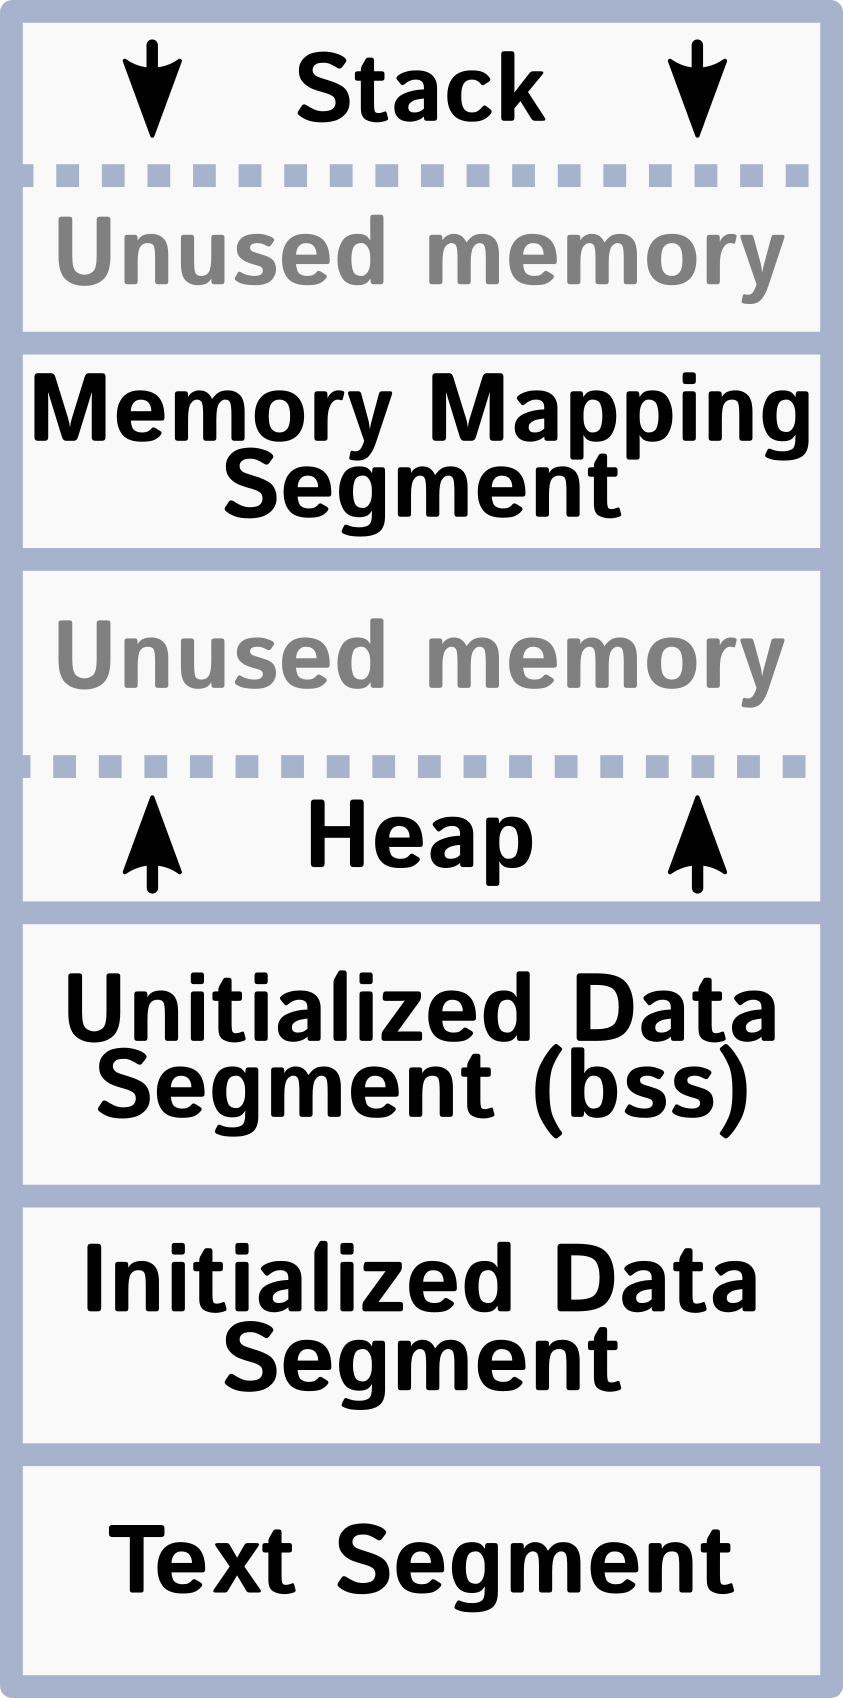
\includegraphics[width=.20\textwidth]{memory_segment} 
  \caption{Segmento de memória}
  \label{fig:memory_segment} 
\end{figure}

A Figura \ref{fig:memory_segment} ilustra seis segmentos de memória diferentes
representando o \emph{layout} de um processo após a criação dele por parte do
SO (essa estrutura pode variar de acordo com a arquitetura). O
\boldAndIndex{segmento de texto} (\emph{Text Segment}) representa a região da
memória que mantém o código executável (compartilhável de somente leitura). Já
o \boldAndIndex{segmento de dados inicializáveis} (\emph{Initialized Data
Segment}) é responsável por manter variáveis estáticas, enquanto o
\boldAndIndex{segmento de dados não inicializados} (\emph{Uninitialized Data
Segment}) mantém variáveis estáticas não inicializadas.  Vale observar que o
segmento de dados não inicializável também é comumente conhecido como
\emph{Block Started by Symbol (BSS)} por causa de um antigo operador usado
pelos montadores \citep{gdb}. O \boldAndIndex{segmento de Mapeamento de
Memória} (\emph{Memory Mapping Segment}) é a região na qual o SO mapeia
arquivos diretamente na memória (e.g.; bibliotecas dinâmicas ou arquivos
especificados pelo programador). O \boldAndIndex{segmento da Stack} compreende
aos dados usados pelo programa durante a execução, como por exemplo, valores de
parâmetros de função, endereço de retorno e variáveis locais (dados
temporários) \citep{silberschatz}.  Por fim, o \boldAndIndex{segmento do Heap}
mantém a memória dinamicamente alocada durante a execução do programa; repare
que o \emph{stack} e o \emph{heap} estão em lados oposto da memória.

O primeiro passo realizado pelo SO quando ele lê o arquivo executável é olhar
para o \emph{header} e obter as informações sobre o tamanho do segmento de
texto e dados. Em seguida, com base nas informações obtidas do \emph{header}, o
SO cria um novo espaço de endereçamento (\emph{Address Space}) com tamanho de
memória suficiente para os segmento de texto e dados. Após alocar memória, o
próximo passo consiste em copiar toda a região de código e dados lidas do
arquivo binário para a memória recém alocada; complementarmente, é feita a
inicialização de todos os registradores e os devidos ajustes no \emph{stack
pointer}. O processo tem o seu \emph{Program Counter} (PC) ajustado para a
função \emph{main} do programa \citep{patterson}, por fim, o SO insere o novo
processo na fila do escalonador.

\begin{figure}[!h]
  \centering
  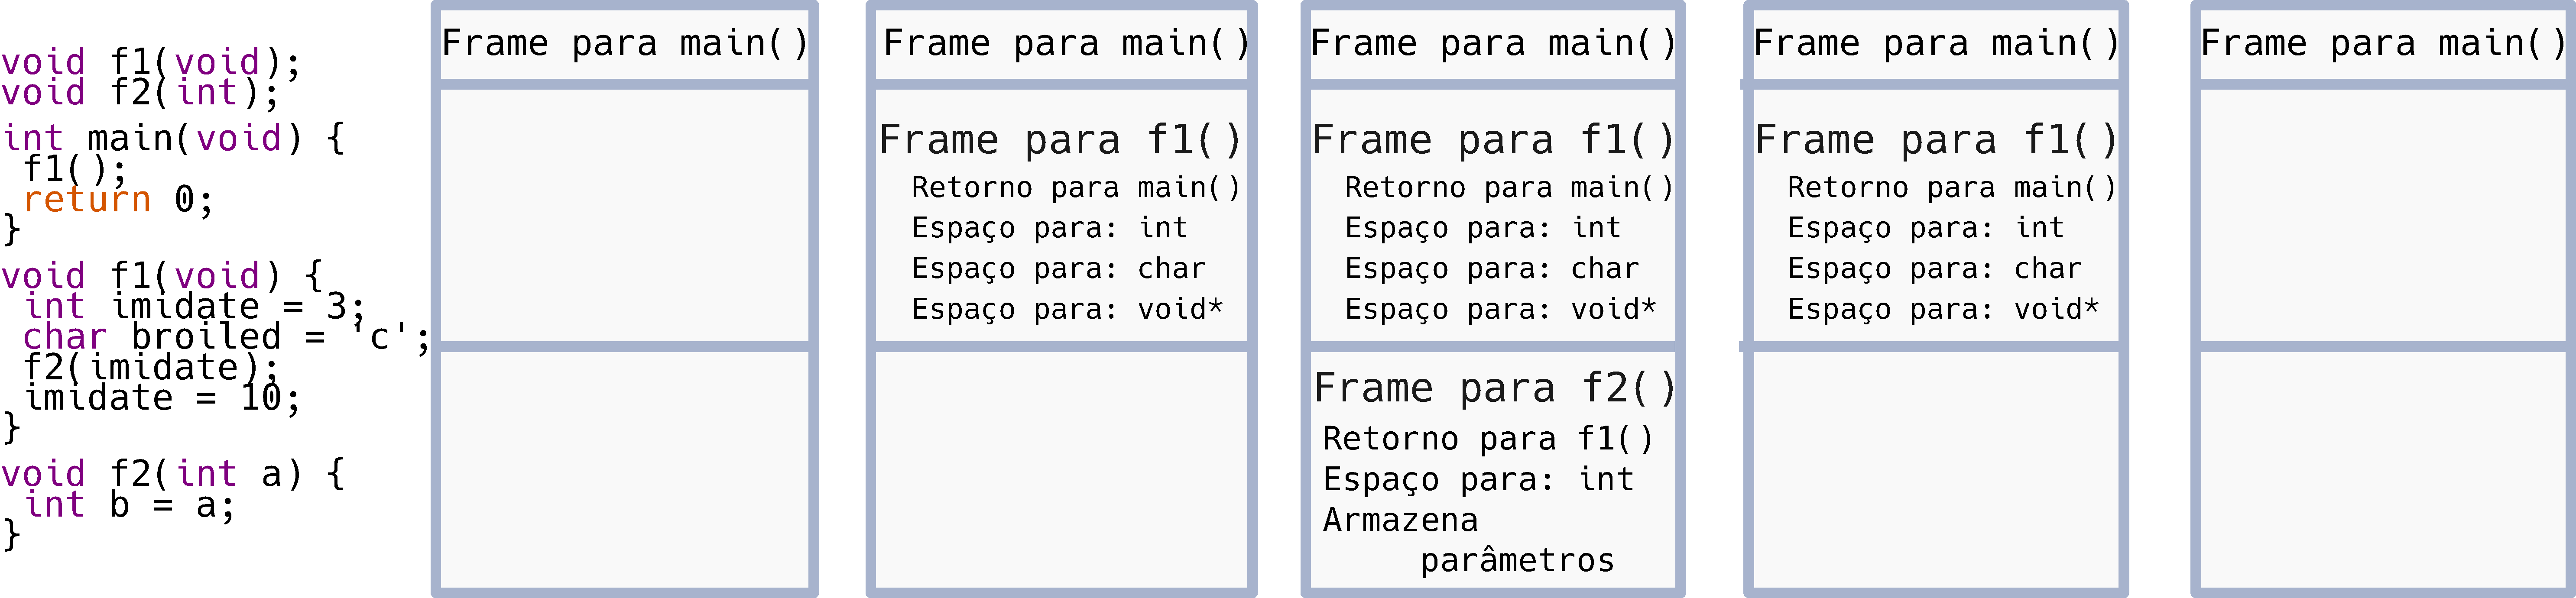
\includegraphics[width=\textwidth]{stack_frame}
  \caption{Alocação e desalocação de Stack frames considerando o padrão CDECL~\citep{patterson}}
  \label{fig:stack_frames} 
\end{figure}

% TODO: Fazer uma ponte melhor do PC com a execução

A \emph{stack} é organizada em uma coleção de \boldAndIndex{Stack Frames}. Toda
vez que uma função é chamada ela cria um novo \emph{frame} que mantém as
variáveis locais, argumentos e o ponto de retorno relacionado a função. Um
processo pode invocar um grande número de funções durante a sua execução,
consequentemente, cada função chamada recebe um \emph{stack frame}. A Figura
\ref{fig:stack_frames} ilustra a alocação e desalocação de \textit{frames} em um simples
programa~\citep{gdb}. No começo, só existe um \emph{stack frame} associado no
topo da função \texttt{main}. Quando uma função local é chamada, o SO vai
alocar um novo \emph{stack frame} no topo do \emph{frame} da \texttt{main},
esse procedimento permite que a execução do processo ocorra de forma
consistente. No fim da execução da função, ela retorna para o ponto na qual a
função foi invocada e o processo de preencher e esvaziar a \emph{stack}
continua.

Todos os processos são descritos por meio de uma estrutura de dados chamada de
\boldAndIndex{Process Control Block (PCB)}, essa é responsável por manter
informações referentes ao status do processo, \emph{program counter} (PC),
registradores da CPU, informações sobre escalonamento, dados sobre contas de
usuários, status de operações de I/O e assim por diante~\citep{silberschatz}.
Uma dos principais motivos para a PCB existir é o conceito de \textbf{troca de
contexto}, responsável por colocar e tirar processos para executar em uma CPU.
Por exemplo, se o usuário dispõe de vários processos rodando ao mesmo tempo, o
SO deve alternar entre todos eles para que cada processo tenham a oportunidade
de executar por um intervalo de tempo. O SO realiza o processo de troca em duas
etapas gerais: (1) salva a PCB atual do processo e (2) carrega a PCB do outro
processo. Em poucas palavras, a troca de contexto deve ser rápida uma vez
que esta não faz nenhum processamento considerado útil.

O conceito apresentado acima revela uma característica de isolamento associada
com a forma na qual os processos funcionam; normalmente, segurança e
estabilidade são positivamente afetadas pelo isolamento de processos. Por outro
lado, existem situações que demandam que os processos cooperem entre si. Para
estes casos é possível notar algumas das desvantagens inerentes a estratégia de
processos atual. Para resolver parte desse problema, algumas bibliotecas ou
chamadas de sistemas são fornecidas como uma interface para coordenar a
interação entre processos executando concomitantemente, esses são conhecidos
pelo nome de \boldAndIndex{Interprocess Communication} (IPC). Por exemplo,
desenvolvedores podem utilizar IPC para compartilhar dados, melhorar o
desempenho das aplicações, modularizar ou por alguma questão de conveniência da
sua aplicação. O IPC tem três limitações principais: elevam o consumo de
memória, adicionam sobrecargas extras de comunicação e tem uma certa
complexidade para serem implementadas. Essas limitações são proibitivas em
aplicações com grande demanda computacional.

\begin{figure}[!h]
  \centering
  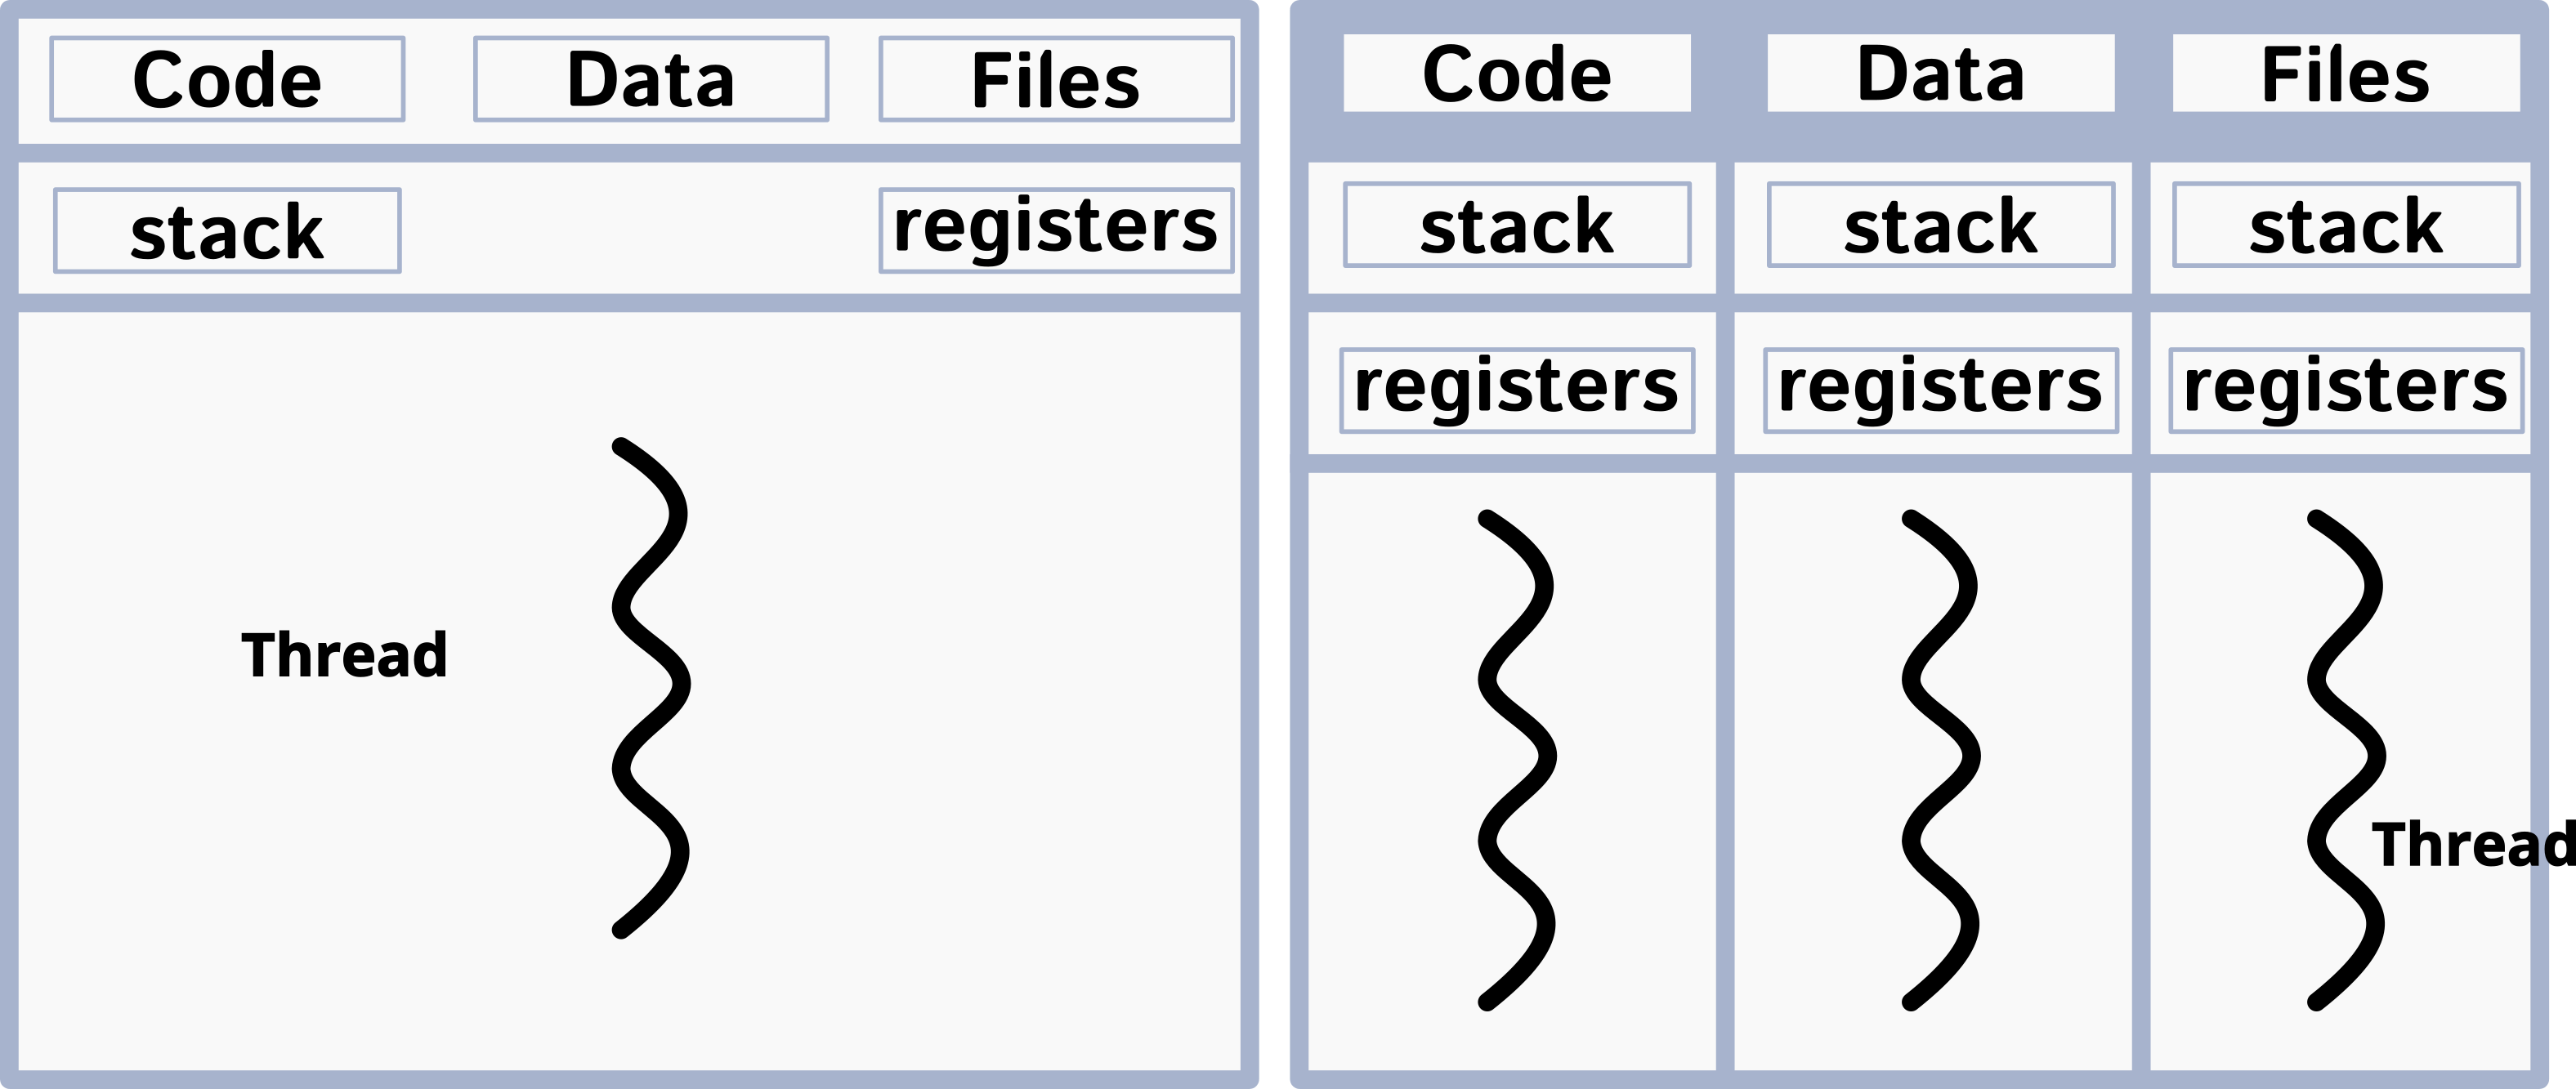
\includegraphics[width=.7\textwidth]{process_and_threads.png}
  \caption{Única thread e multi-thread~\citep{silberschatz}}
  \label{fig:single_thread_multi_thread}
\end{figure}

Como é possível perceber, processos são abstrações poderosas com algumas
limitações, principalmente ao que se refere ao desempenho e complexidade. Além
disso, processos têm apenas um fluxo de execução (\textit{thread}) para
realizar todo o trabalho. Naturalmente os desenvolvedores buscam atingir mais
paralelismo ou concorrência por meio de IPC, contudo os programadores precisam
lidar com as sobrecargas extras impostas por essa estratégia. Por esse
motivo, buscou-se por muito tempo por formas de elevar o desempenho das
aplicações por meio de melhorias no grau de paralelismo. Como resultado direto
de tal esforço surgiu o conceito de um processo ter múltiplas \emph{threads}
compartilhando praticamente todos os elementos básicos com exceção da
\emph{stack} e do PC. A Figura \ref{fig:single_thread_multi_thread} mostra um
processo com uma \emph{thread} e outro com múltiplas \emph{threads}, note na
figura o isolamento da \emph{stack} e do PC.

\lstinputlisting[
                 language=C,
                 caption={Exemplo simple de threads},
                 label={lst:simplethreads}
                ]{code/simpleThread.c}

\begin{lstlisting}[frame=single,
                   language=bash,
                   caption={Saída do exemplo de threads},
                   label={lst:simpleThreadOutput}]
$ ./example 
Thread 1 
Thread 2
$ ./example
Thread 2 
Thread 1
\end{lstlisting}

O Código \ref{lst:simplethreads} ilustra o comportamento básico das
\emph{threads} por meio de uma biblioteca chamada de \emph{POSIX Thread Library
(Pthread)}. Veja no Código a criação de duas novas \emph{threads} que mostram
mensagens simples, note também que a implementação tem três \emph{threads}
diferentes: a \emph{thread} principal associada ao processo e outras duas
\emph{threads} diferentes criadas após a função \texttt{main()} iniciar a sua
execução. A função \texttt{thread\_kernel()} tem o código que é executado por
cada nova \emph{thread} criada na função principal. Note que
\texttt{thread\_kernel} recebe um ponteiro genérico, converte esse para um tipo
\texttt{char *} e mostra o valor no final.

A função \texttt{main()} declara duas variáveis do tipo \texttt{pthread\_t}, que
são responsáveis por manter as informações referêntes as \emph{threads}.
Adicionalmente, são declaradas duas \emph{strings} de mensagens para serem
mostradas posteriormente dentro das \emph{threads} criadas. Quando o programa
chega na função \texttt{pthread\_create()}, a biblioteca solicita ao SO a
criação de uma nova \emph{thread} que executa a função \texttt{thread\_kernel}
em paralelo. A função \texttt{pthread\_create()} é chamada novamente e cria a segunda
\emph{thread} de execução baseada na função \texttt{thread\_kernel}, contudo,
com outra mensagem associada com ela. O código termina com a função
\texttt{pthread\_join()}, que mantém a \emph{thread} princípal até que as duas
\emph{threads} terminem a sua execução. A saída ilustrada em
\ref{lst:simpleThreadOutput} mostra as duas execuções que aconteceram em
paralelo, isso pode ser percebido pela sequência não determinística da saída. A
diferença na sequência é explicada pela variação imposta pelo escalonador.

\begin{figure}[!h]
  \centering
  \includegraphics[width=.60\textwidth]{theads_and_stack} 
  \caption{Stack com duas threads}
  \label{fig:stack_threads} 
\end{figure}

Para a melhor compreensão de como o SO trata o Código \ref{lst:simplethreads}
durante a execução, veja a Figura \ref{fig:stack_threads} ilustrando o que
acontece da perspectiva do processo. Como esperado, o segmento de texto e dados
é compartilhados entre as \emph{threads}. A principal mudança pode ser
observada no segmento da \emph{stack}, toda vez que uma nova \emph{thread} é
criada um novo segmento de \emph{stack} é gerado; a independência entre
\emph{threads} é assegurada por multiplas \emph{stacks} isoladas. Toda vez que
a \emph{thread} é mudada, o \emph{stack pointer} e os registradores são
atualizados.

\section{Gerenciamento da Memória relacionada aos processos}

% TODO: Merge com a próxima seção
Fazer com que a memória do sistema esteja disponível e utilizável para uma
aplicação representa uma das principais responsabilidade de um SO. A maioria
dos SOs oferece a ilusão de que toda a memória está acessível para o processo,
isso é possível devido ao desacoplamento da memória física de como um processo
a vê. Processos só veem o \emph{Virtual Address Space (VAS)} e por sua vez, esse
é mapeado por um SO (com auxílio de hardware) para uma memória física o que
garante um bom isolamento entre processos. Para manipular VASes e oferecer um
recurso útil para a aplicação do usuário, os SOs tem que adotar um modelo de
memória especifica; atualmente, a maioria dos SOs de produção e hardware
suportam amplamente o modelo de gerenciamento de páginas.  Esse modelo separa a
VAS e o espaço de endereçamento físico para cada processo em um conjunto de
páginas, essas tem um pequeno intervalo contíguo de endereços, tamanho fixado,
endereço de início e permissões. O modelo de paginação tem algumas vantagens:
controle das permissões no nível da página, mecanismos de compartilhamento,
rápida verificação de proteção, notificações acuradas sobre violações e a
possibilidade de mapear memória em disco.

\subsection{Endereços lógicos, físicos e Paginação}

% TODO:  Nessa seção, não temos a intenção de discutir profundamente os mecanismos presentes 

Imagine um programa escrito em C, em algum momento do código esse faz uma
alocação de memória e em um outro momento essa região é lida ou escrita. Esse
programa de alto nível é traduzido para um conjunto de instruções de baixo
nível na qual a CPU consegue manipular, o arquivo contendo essas informações é
comumente chamada de binário.  Posteriormente esse binário é carregado pelo SO
e o programa começa a sua execução. Durante a realização das tarefas da
aplicação, naturalmente ocorrem acessos aos endereços de memória. Da relação
entre o código de alto nível, o binário e o acesso a memória, surgem algumas
questões, dentre elas: como o programa consegue acessar o endereço sem conhecer
as características da máquina? Como os programas evitam os acessos aos mesmos
endereços?

A resposta para as perguntas acima nascem de três conceitos: \textit{address
binding} em tempo de execução, espaço de endereçamento e paginação. O processo
de "construção" do endereço nasce durante a compilação do código fonte, nesse
momento o compilador consegue identificar diversos tipos de acesso a memória
(não entraremos em detalhes, por fugir do escopo desse trabalho) e este faz uma
marcação em certos endereços que indicam que o mesmo deve ser definido em tempo
de execução. Com base nessa "marcação" os SO e o hardware ganham um mecanismo
para definir o endereço em tempo de execução.

Como dito anteriormente, o binário contém certas informações necessárias para a
criação do processo e também para a definição de acesso de um endereço. Quando
o software começa a sua execução, significa que a CPU está executando as
instruções descritas no binário, dentre elas as tentativas de acesso a certos
endereços na memória.

Todo endereço gerado pela CPU recebe o nome de \boldAndIndex{endereço virtual} ou
\textbf{endereço lógico}\index{Endereço lógico}, por sua vez, o conjunto desses
endereços recebe o nome de \boldAndIndex{espaço de endereçamento virtual (Virtual
Address Space)} ou simplesmente VAS. De forma simplificada, podemos dizer que
esses endereços gerados pela CPU não são válidos da perspectiva da memória,
i.e., são apenas endereços usados pela aplicação mas que não correspondem ao
endereço real da memória física. Os endereços reais da memória são chamados de
\boldAndIndex{endereços físicos} e o conjunto de todos os endereços da memória são
chamados de \boldAndIndex{espaço de endereçamento físico}. Agora você deve está se
perguntando: qual a relação entre esses dois tipos de endereços? Como eles
ajudam a resolver os problemas citados no começo? Eis que surge um terceiro
elemento entre esses conceitos, o \textit{Memory-Management Unit
(MMU)}\index{MMU}. Veja a Figura \ref{fig:mmu} ilustrando a posição "física"
desse hardware:

\begin{figure}[!h]
  \centering
  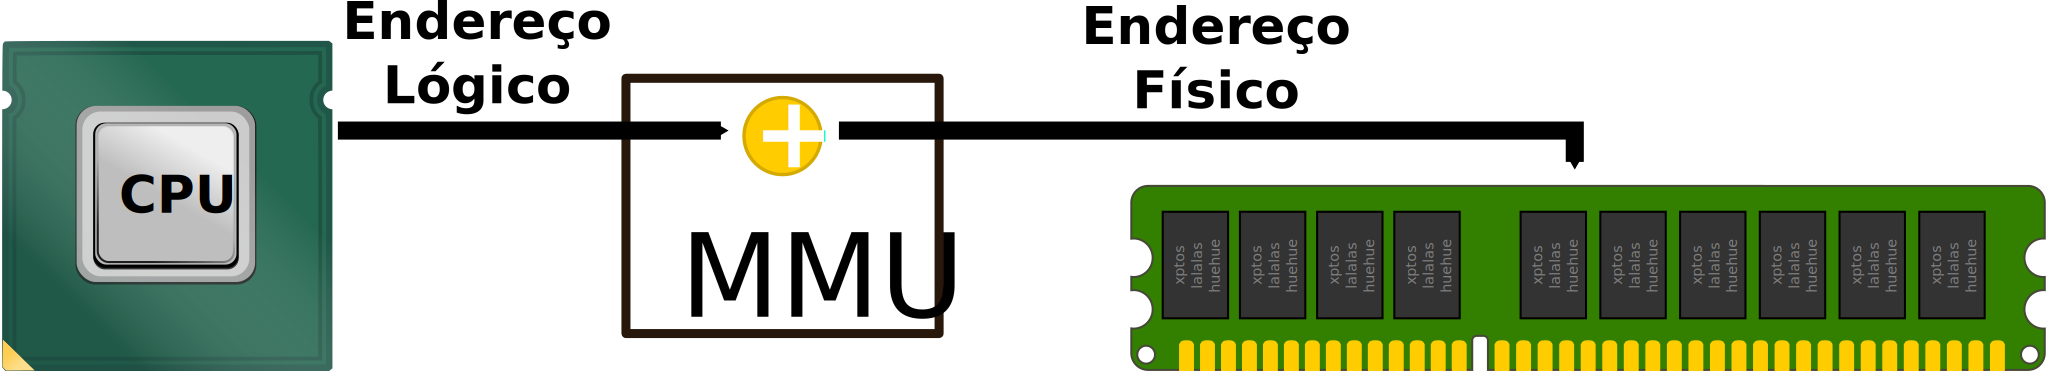
\includegraphics[width=\textwidth]{mmu} 
  \caption{Representação didática da MMU}
  \label{fig:mmu}
\end{figure}

A MMU é um hardware usado para fazer o mapeamento do endereço virtual para o
endereço físico em tempo de execução. A Figura \ref{fig:mmu} mostra a CPU
gerando um endereço, que por sua vez é entregue a MMU. A MMU converte o
endereço virtual em um endereço físico e procede com o acesso a memória. Dado a
visão geral do que acontece do endereço virtual para o endereço físico com o
intermédio da CPU, podemos olhar com mais detalhes o funcionamento do
mapeamento e introduzir o conceito de paginação.

Antes de nos aprofundarmos na paginação, vale a pena fazer uma última reflexão
sobre os endereços físicos e virtuais. Começando com os endereços virtuais,
repare que esses precisam ter algum intervalo definido e que seja finito, qual
seria? Esse intervalo começa em 0 e vai até um valor máximo definido em um
conjunto de bits chamado de \textit{virtual bits}. Durante muito tempo, o total
de bits era de 32 o que dava um espaço de endereçamento de 4 Gb; hoje em dia é
relativamente simples encontrar CPUs com 48 bits o que gera uma VAS de 256 TiB.
Na prática, isso significa que um software executando em um SO moderno tem a
ilusão de que pode acessar todos os endereços fornecidos pela VAS. Por
enquanto, sabemos que isso não é verdade, pois dificilmente conseguimos
fornecer tanta memória. Por esse motivo e como ilustrado na Figura
\ref{fig:vas_pas}, notamos que o endereço virtual é várias vezes maior do que o
endereço físico. Para piorar, a memória física deve ser compartilhada entre
vários processos em execução no SO.

\begin{figure}[!h]
  \centering
  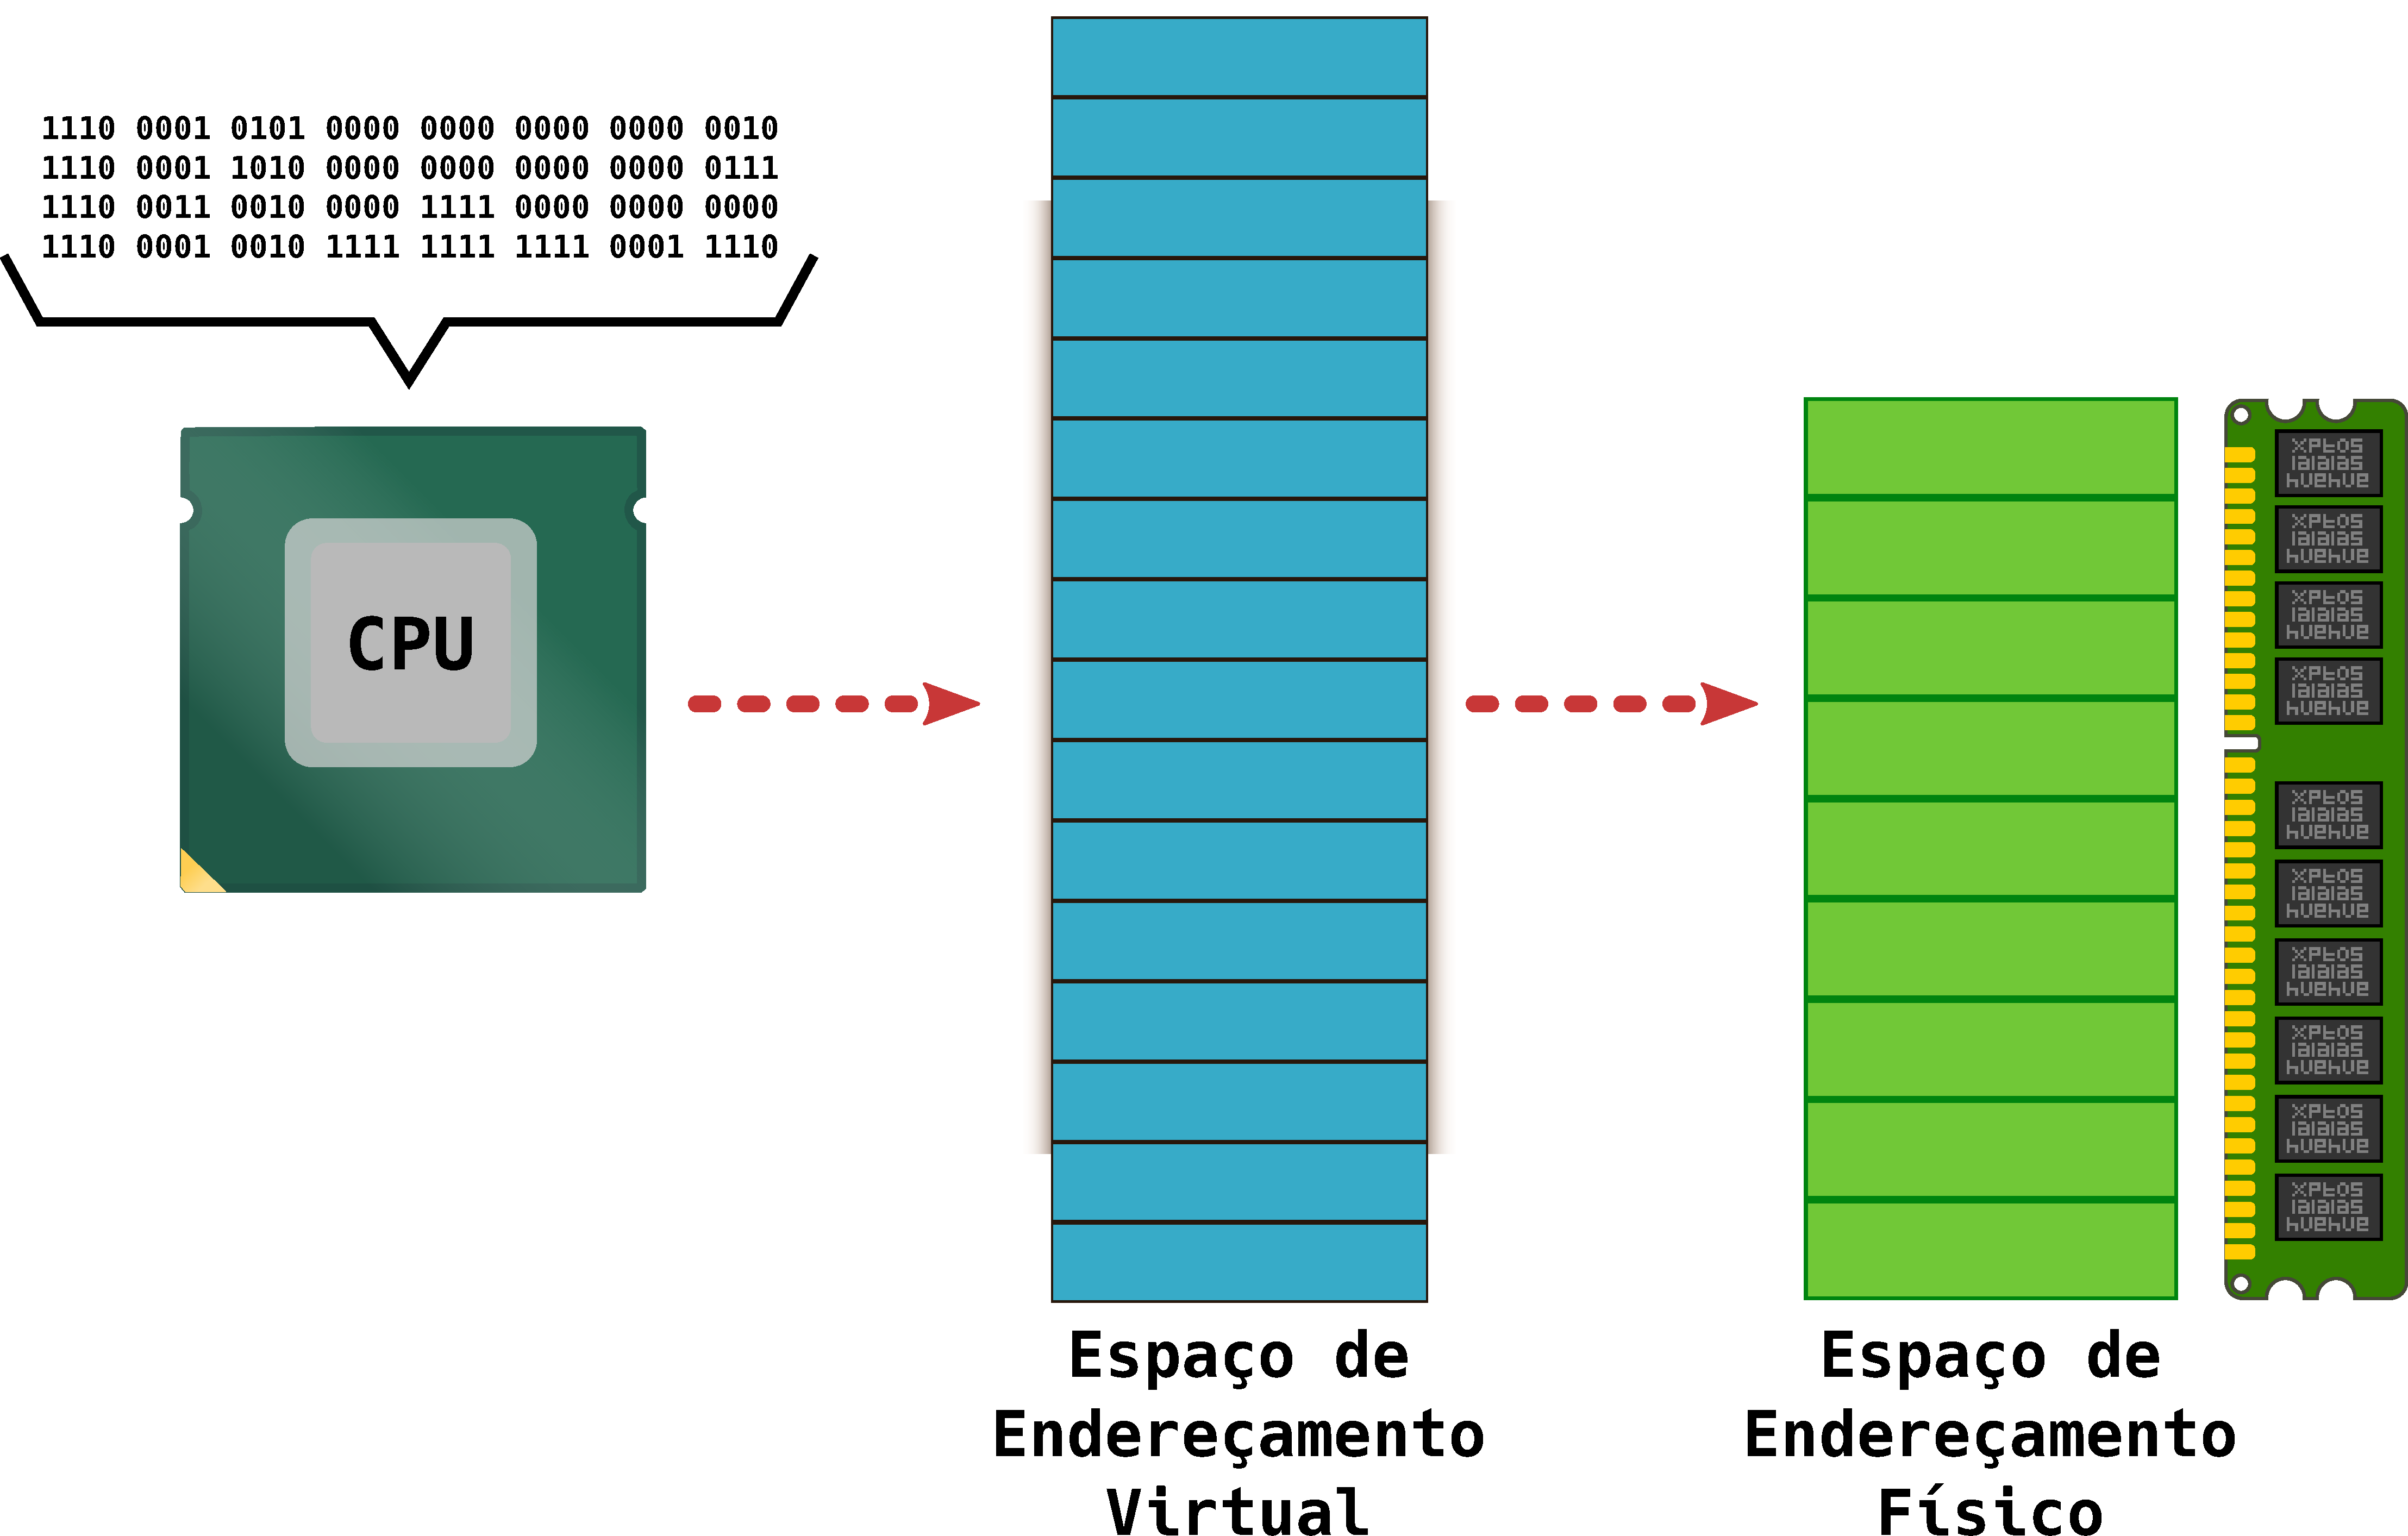
\includegraphics[width=\textwidth]{virtual_vs_fisico} 
  \caption{Espaço de endereçamento virtual vs. físico}
  \label{fig:vas_pas}
\end{figure}

O modelo de paginação é um esquema que surge com o objetivo de permitir que os
endereços físicos do processo possam ser dispostos na memória de forma
não-contínua. A implicação direta desse modelo é a de que um processo não
precisa estar totalmente na memória e que esse conceito se sustenta para "n"
processos. Contudo, para que tal modelo possa ser implementado, é preciso
dividir o espaço de endereçamento virtual e físico em \boldAndIndex{páginas} e
\boldAndIndex{frames} respectivamente. Uma vez que ambos os espaços de endereçamentos
são subdivididos, é necessário ter um mecanismo para saber o que está presente
ou não na memória. Para ter uma visão de como todo o modelo de paginação
funciona, veja a Figura \ref{fig:paginacao}.

\begin{figure}[!h]
  \centering
  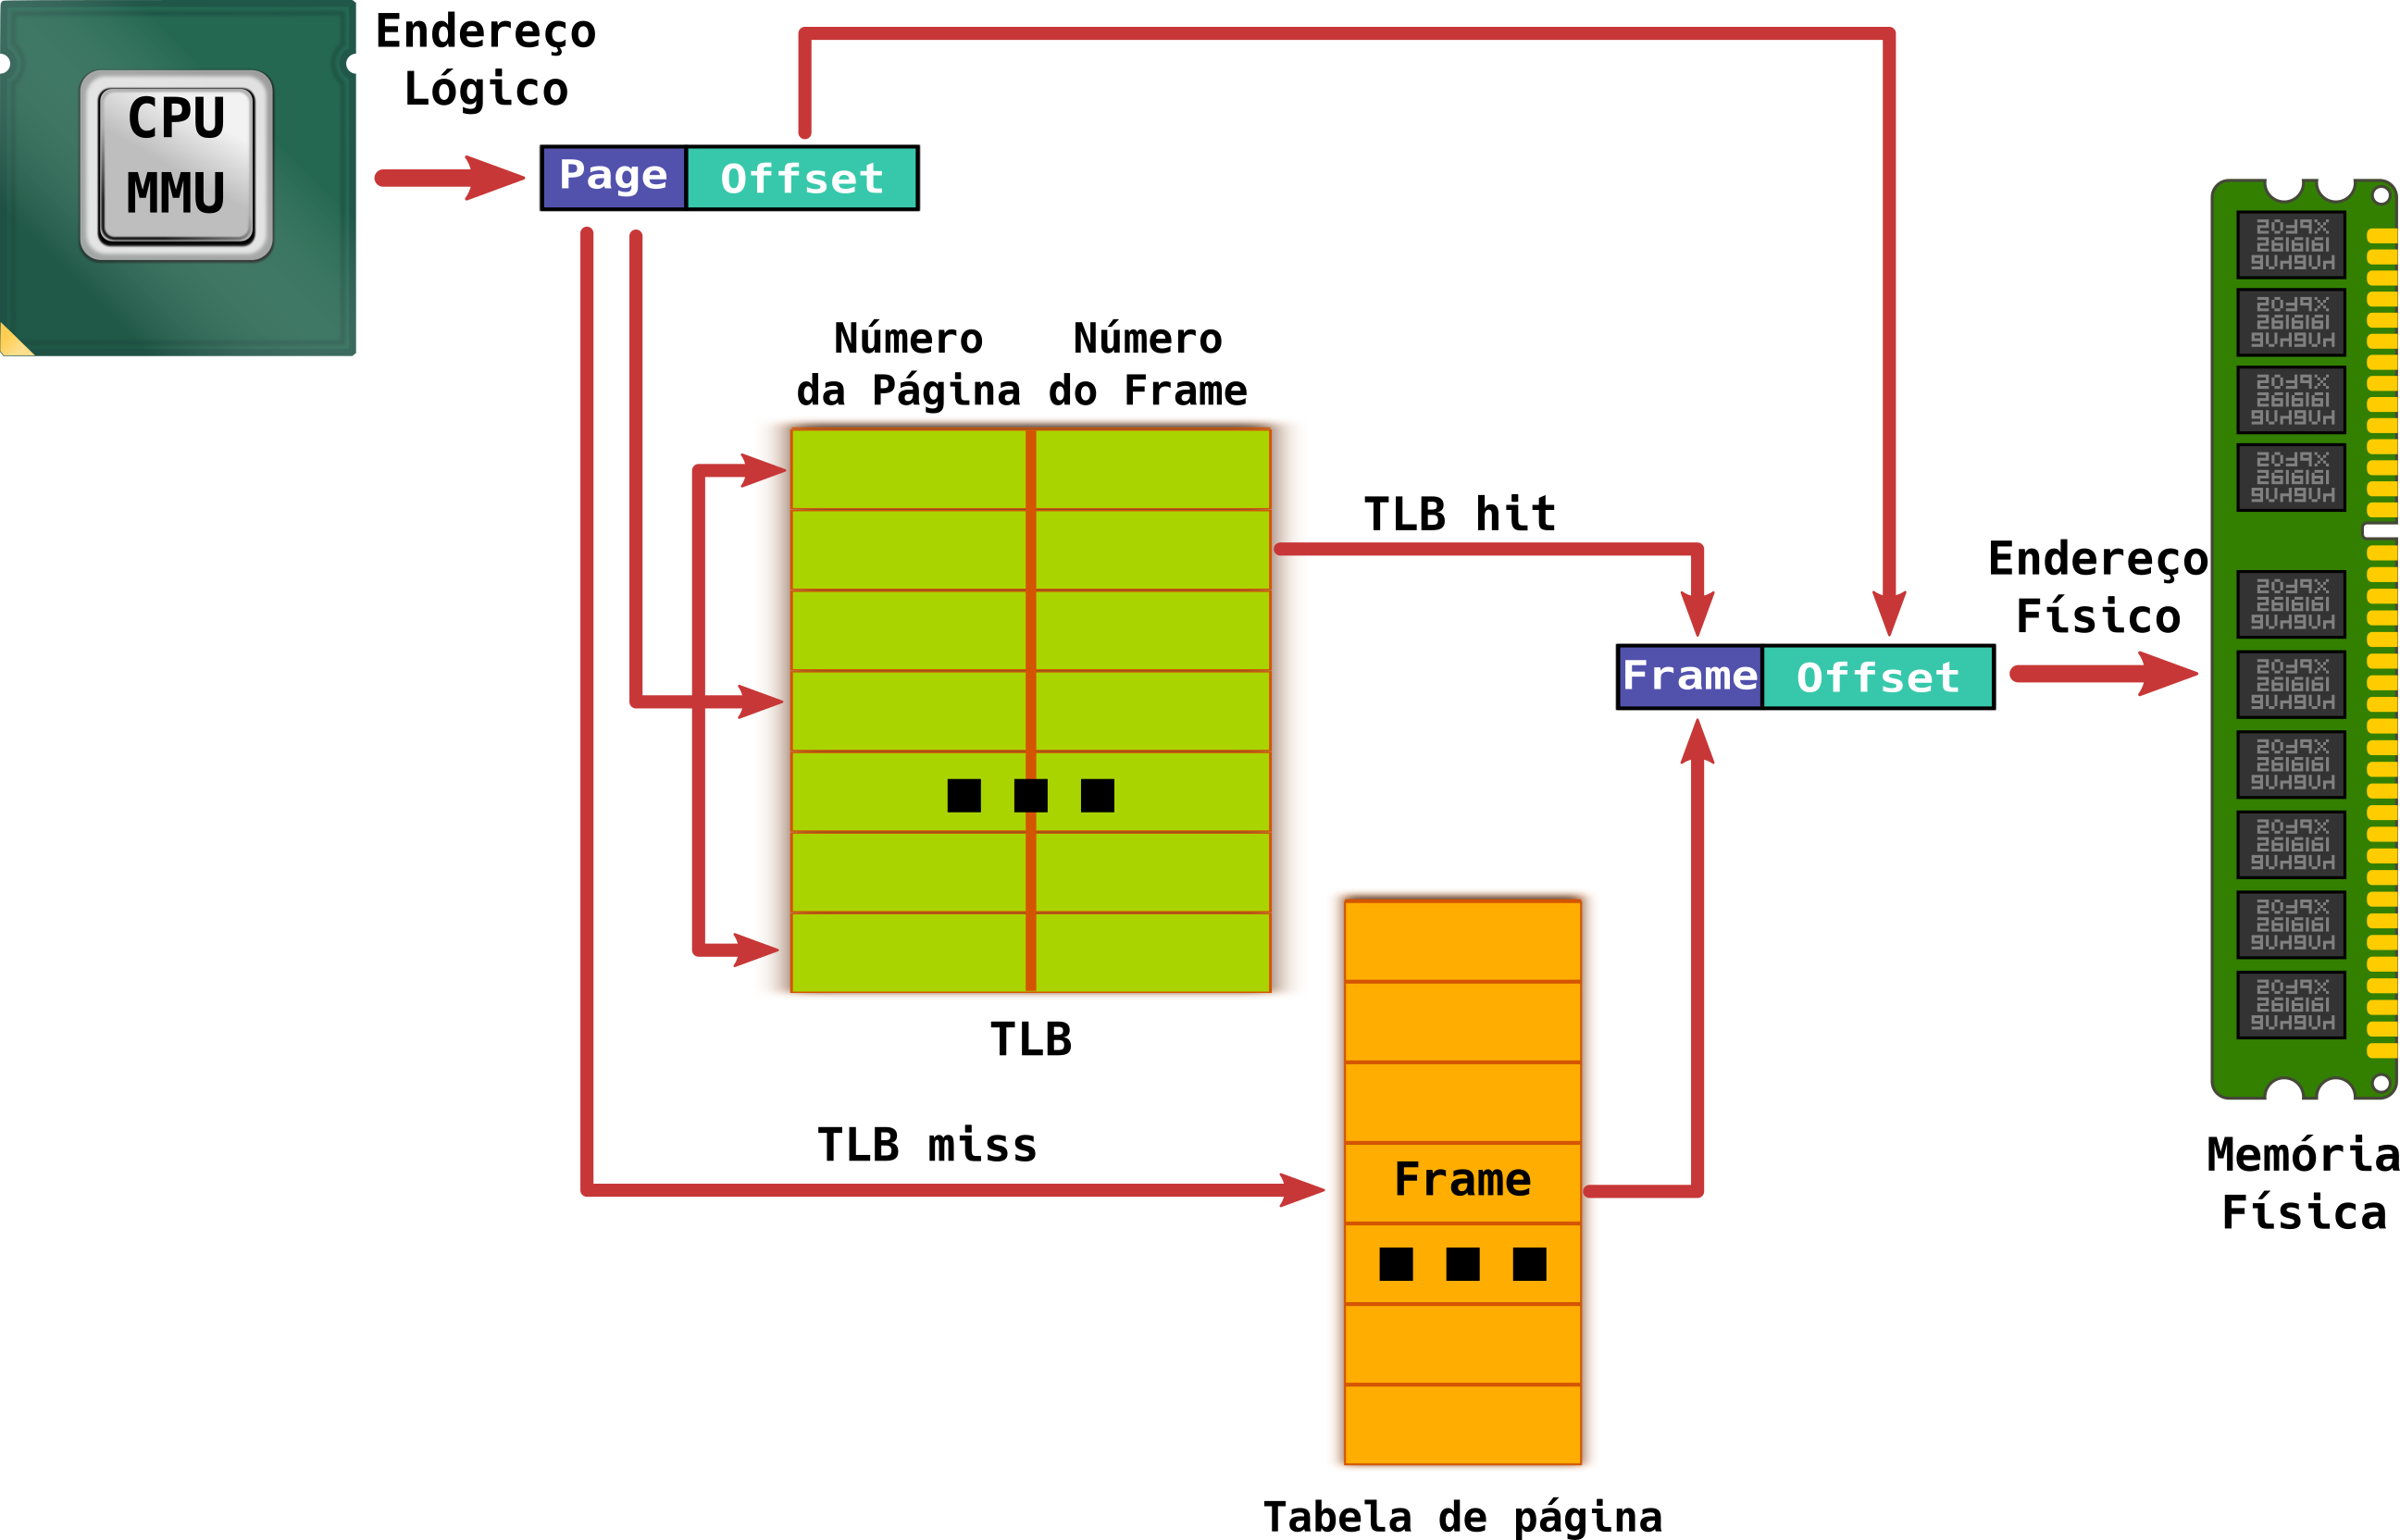
\includegraphics[width=0.8\textwidth]{paginacao} 
  \caption{Modelo de paginação}
  \label{fig:paginacao}
\end{figure}

Na Figura \ref{fig:paginacao} observamos que a CPU gera um endereço lógico, por
sua vez esse endereço é subdividido em duas partes: um \textit{page} e um
\textit{offset}. O page comporta-se como um index corresponde a uma entrada em
uma estrutura de dados chamada de \boldAndIndex{Tabela de Paginação}, essa tabela faz
parte da abstração de processos e tem uma entrada especificada na PCB, ou seja,
todo processo tem tal tabela associada a si. Cada entrada na tabela corresponde
ao endereço de início de um frame na memória que está associado ao processo.
Para ilustrar melhor esse conceito, imagine um programa que aloca espaço na
memória, na prática o SO cria uma nova entrada na tabela e retorna o endereço
virtual para a aplicação.  Depois que o valor referente ao index é recuperado a
MMU soma o \textit{offset} da segunda parte do endereço virtual e finalmente o
acesso a memória física ocorre.

\begin{figure}[!h]
  \centering
  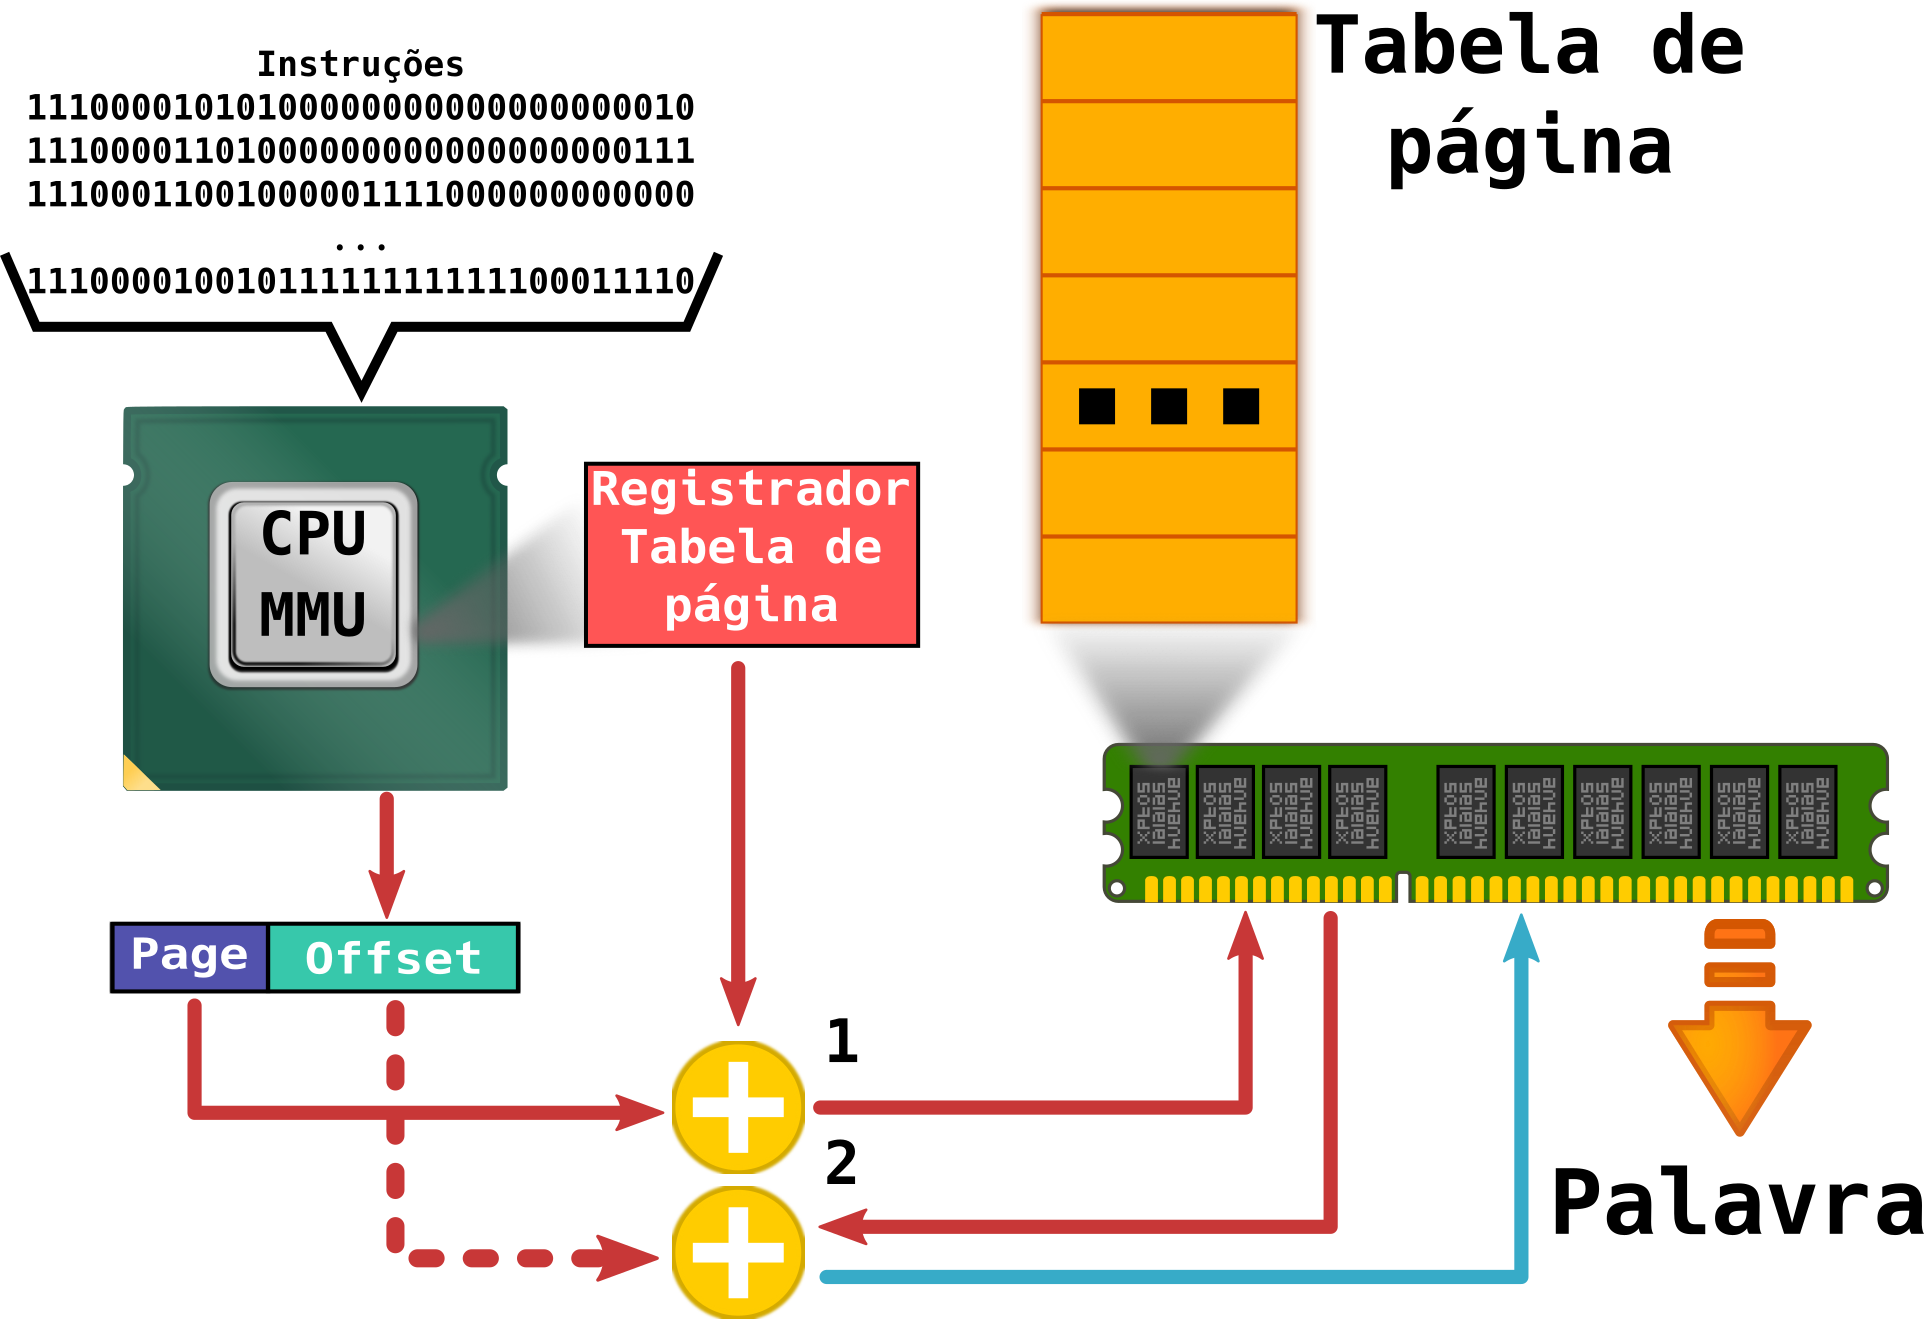
\includegraphics[width=0.8\textwidth]{paginacao_passos} 
  \caption{Passos do acesso a memória com paginação}
  \label{fig:passos_paginacao}
\end{figure}

A Figura \ref{fig:passos_paginacao} exemplifica o processo descrito
anteriormente. Repare que são necessários vários acessos a memória para
construir o endereço final e finalmente conseguir acessar a palavra de dados,
claramente isso não é eficiente. Nesse sentido, existe um mecanismo que busca
reduzir esses acessos por meio de uma tabela chamada de \boldAndIndex{Translation
look-aside Buffer (TLB)}. Essa tabela salva o último acesso (coluna e valor)
feito a tabela de páginas evitando que a memória seja consultada inúmeras
vezes. Tal mecanismo é ilustrado na Figura \ref{fig:paginacao}, note que a
busca na TLB e na tabela de página ocorre em paralelo, se a TLB tiver um acerto
a procura na da memória; do contrário, \textit{TLB Miss}, a busca na memória já
se inciou.

Por fim, é importante destacar que os mecanismos descritos nessa seção trazem
inúmeros benefícios diretos e indiretos. Talvez as vantagens mais direta seja a
possibilidade de ter o processo na memória de forma não contígua e assim
conseguir controlar o que deve ou não estar presente na memória. Indiretamente,
esses mecanismos isolam cada processo de acordo com a VAS uma vez que todo
processo tem a ilusão de que tem total controle da memória. Além disso, o
mecanismo de paginação facilita a operação de realizar o compartilhamento de
dados entre os processos; o SO orquestra um conjunto de páginas com a mesma
visibilidade (indicada pelo programa no espaço de usuário) para ser
compartilhado entre processos.

\subsection{Modelo de Segmentação}

Além do mecanismo de gerenciamento de memória fornecido pela paginação, também
existe uma alternativa chamada de segmentação. Esse modelo divide o memória
referente ao programa de acordo com as suas seções, empiricamente esse modelo
comporta-se dividindo programa em um conjunto de segmentos, por exemplo, uma
área para o \textit{text}, outra para os dados, \textit{stack}, etc. Os
tamanhos de cada segmento podem ser variáveis, o que leva a uma visão
bidimensional da memória uma vez que os endereços passam a ser construído como
uma tupla: \\

\texttt{<número do segmento, offset>}~\citep{silberschatz}.

O modelo de segmentos oferece uma visão bidimensional, mas a memória continua
sendo linear, por isso é necessário converter os endereços.
A Figura G mostra como a segmentação funciona com o suporte de hardware, repare
que o endereço gerado pela CPU é dividido em duas partes. A primeira parte do
endereço corresponde ao número do segmento salvo na tabela de segmentos, por
sua vez, o valor associado ao index é um endereço presente na memória física.
Como ilustrado na figura, a tabela de segmentos tem dois valores: limite e
base. O limite é o tamanho máximo do segmento e é usado para verificar se o
offset passado é valido. O segundo valor, base, é o começo do segmento na
memória física. Se tudo estiver certo, o endereço final é acessado utilizando a
soma do valor base com o offset.

\begin{figure}[!h]
  \centering
  \includegraphics[width=.80\textwidth]{segmentacao} 
  \caption{Segmento de memória}
  \label{fig:memory_segment} 
\end{figure}

Tanto o modelo de segmentação quanto o de paginação tem suporte de hardware. O
Windows é um SO que faz uso do modelo de segmentação, enquanto o MacOS e o
GNU/Linux usam a paginação. Como a CPU costuma dar suporte para ambos os
esquemas, os SOs podem utilizar esses mecanismos para executar aplicações de
outros SOs. Por exemplo, o Wine executa aplicações Windows no Linux utilizando
parte dos recursos de segmentação fornecidos pela CPU.

\subsection{Outros Mecanismos de Memória}
\label{sec:outros_mecanismos_memoria}

Os microprocessadores ARM oferecem alguns recursos adicionais atrelados a
tabelas de tradução, dentre eles destacam-se os campos de permissão e o domínio
(estes trabalham juntos). Cada região de memória definida na tabela de tradução
é controlada por um domínio que é especificado em um campo da tabela, no total
existem 16 desses domínios diferentes disponíveis para utilização
\citep{armdeveloperguide}. O aspecto mais interessante em se utilizar domínios
está no comportamento que este apresenta caso ocorra alguma tentativa de acesso
da memória, dentre elas:

\begin{itemize}
  \item O acesso pode ser permitido se o conjunto de permissões presentes na
        tabela permitir;
  \item Gerar uma falta de domínio;
  \item O acesso é permitido de acordo com a permissão.
\end{itemize}

Normalmente quem faz a solicitação de acesso a memória é a CPU em favor de
algum processo, então a MMU precisa proceder com algumas verificações que
consiste em três passos:

\begin{enumerate}
  \item A MMU verifica o número do domínio encontrado na tabela de tradução;
  \item Com base no número obtido do passo anterior, a MMU verifica a permissão
        de acesso no registrador de controle de acesso;
  \item De acordo com o valor encontrado no registrador de domínio de acesso a
        MMU pode tomar as seguintes decisões:
  \begin{itemize}
    \item Permitir o acesso;
    \item Bloquear o acesso;
    \item Verificar a permissão de acesso em uma tabela de tradução.
  \end{itemize}
\end{enumerate}

Nesse contexto o SO pode tomar algumas decisões para cada aplicação; dentre
elas permitir, restringir ou negar o acesso para diferentes áreas da memória.
Além disso, o SO pode mudar permissões de acesso para um grande número de
regiões simultâneas. Note que o mecanismo de domínios é um recurso adicional
ao tradicional modelo de controle da memória adotado pelos SOs, ou seja, é
um recurso não fundamental mas que oferece novos recursos aos desenvolvedores.

\subsection{Uma visão prática do programa na memória}
\label{sec:visao_pratica_mem}

A maioria dos conceitos apresentados até agora representam o ponto de vista
teórico dos SOs, nessa seção revisitamos e expandimos alguns dos conceitos da
perspectiva do Kernel Linux. Essa visão é relevante para o presente texto uma
vez que a maioria dos trabalhos analisados faz uso de SOs baseados no Kernel
Linux. Por fim, por uma questão de simplicidades usaremos o termo Kernel como
sinônimo de Linux nessa seção.

Para iniciar a analise, começamos por um fato interessante sobre VAS no Linux
em uma arquitetura x86: uma vez que a VAS é ativada, todo sistema é afetado
incluindo o Kernel. Por este motivo, uma porção da VAS tem que ser reservada
para o Linux de forma a manter o acesso restrito (privilégiado) e sempre
presente na memória física. Por outro lado, a VAS dos processos são movidas
constantemente de acordo com a troca de contexto e podem ser acessados pela
aplicação.

A Figura \ref{fig:vas_contexto} busca ilustrar o mapeamento da VAS levando-se
em consideração o espaço reservado para Kernel e os processos. O lado esquerdo
da figura mostra de forma detalhada a área do Kernel e os segmentos alocados
para o processo em execução (descrito na seção \ref{sec:processos-e-threads}).
A figura também demonstra a troca de contexto que ocorre entre dois processos;
repare que a VAS dos processos é alterada mas o kernel permanece constante.

\begin{figure}[!h]
  \centering
  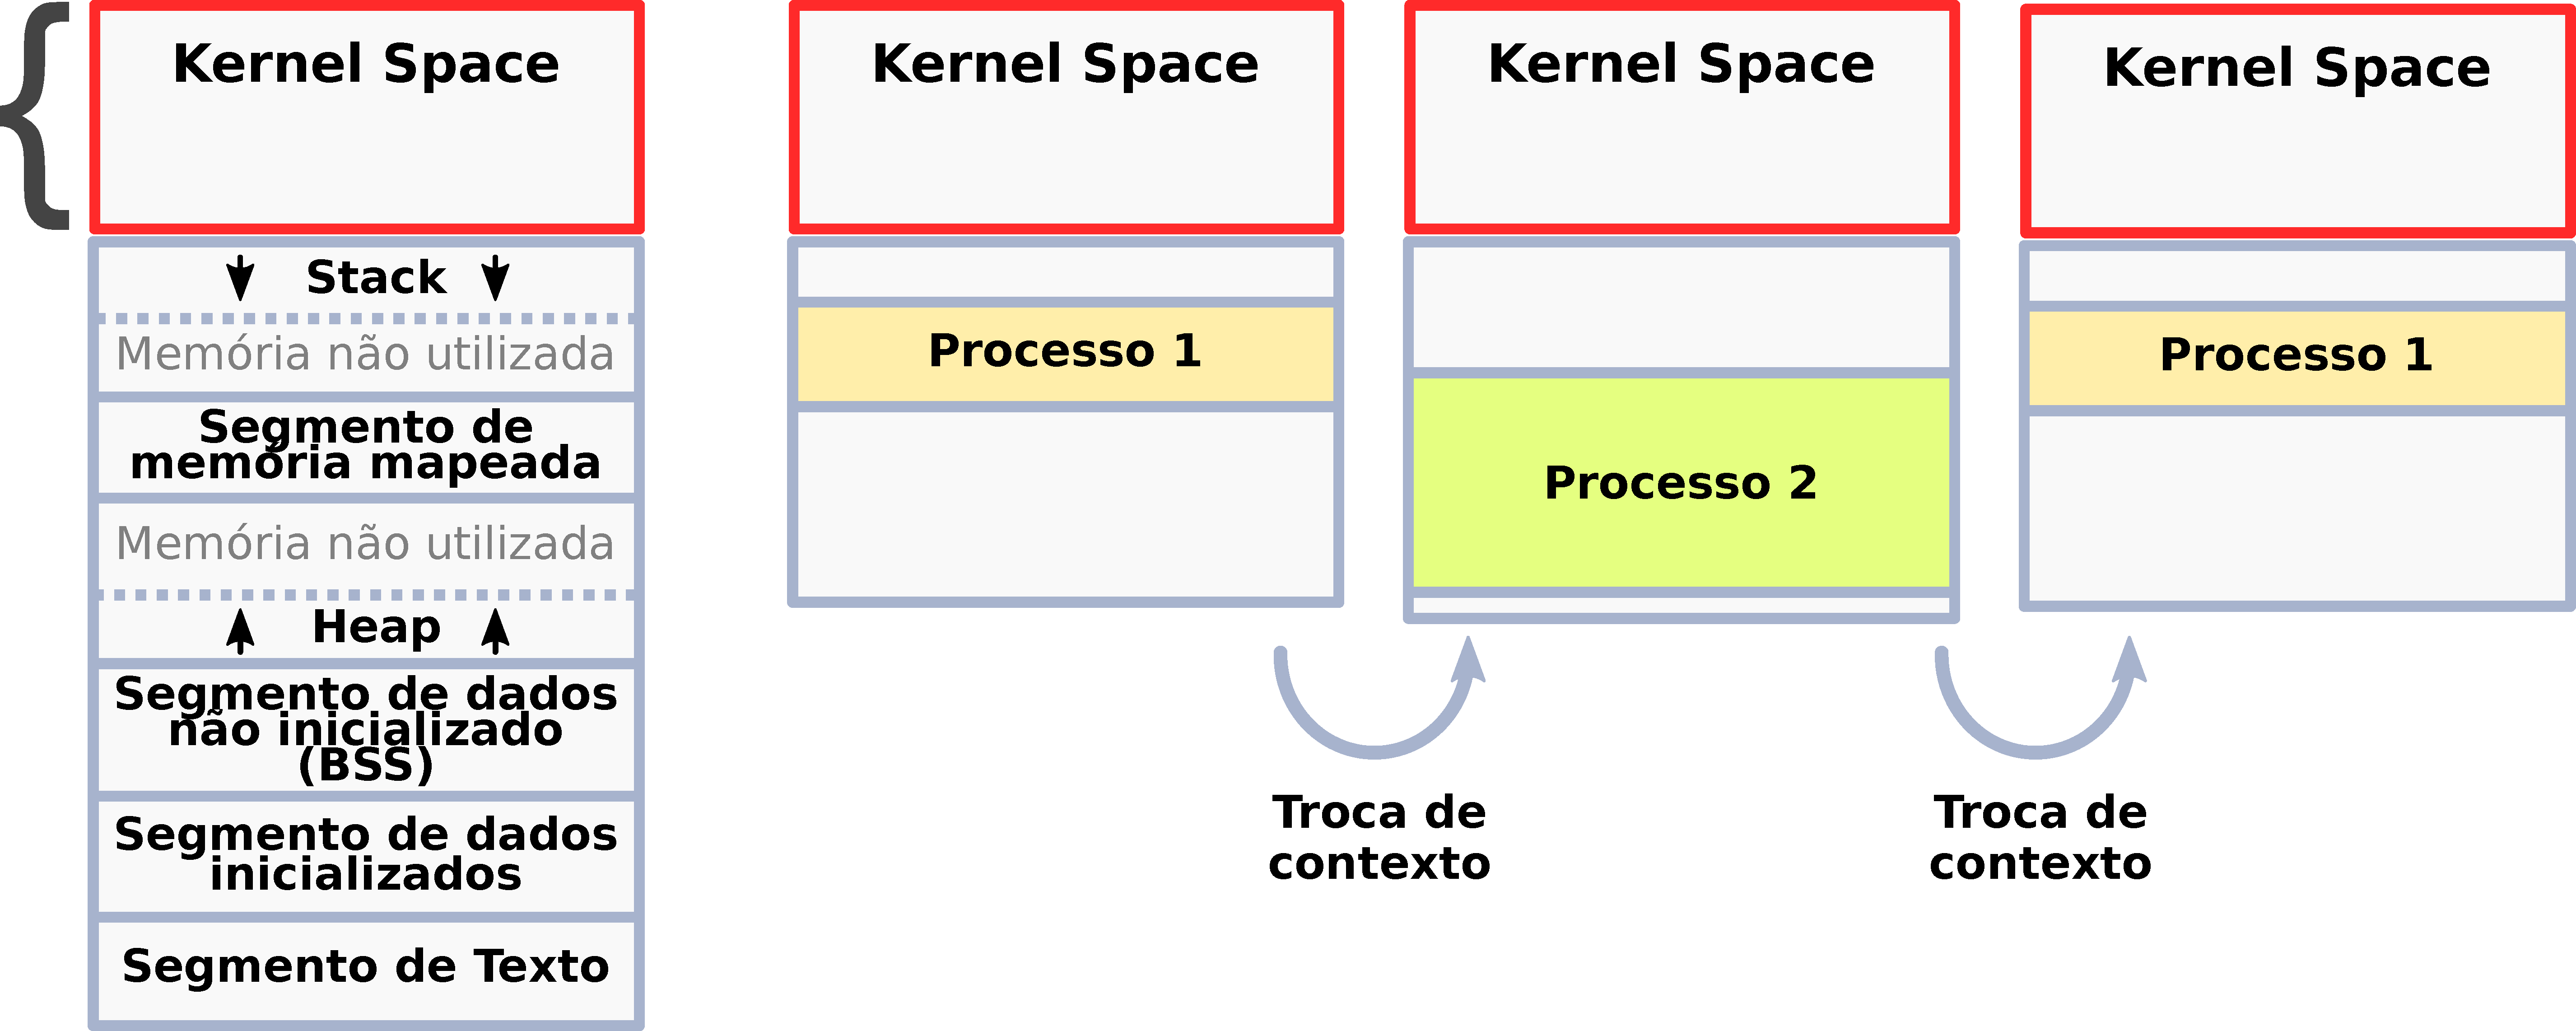
\includegraphics[width=\textwidth]{segmento_troca_contexto}
  \caption{VAS durante a troca de contexto, imagem baseada em \citep{kernel_manages_memory}}
  \label{fig:vas_contexto}
\end{figure}

O \textit{layout} de uma VAS é o mesmo para todos os processos, note que isso
cria brechas de segurança uma vez que um atacante que compreenda essa informação
pode explorar a mesma com o objetivo de realizar ataques. Como resposta a essa
falha de segurança o Kernel implementa uma série de mecanismos de randomização
conhecidos como ASLR, KASLR and KARL~\citep{aslr, kaslr}. Tal recurso faz com
que a sequência dos segmentos sejam randomizada a cada execução do processo,
tornando o sistema mais seguro.

Como explicado na Seção \ref{sec:processos-e-threads}, toda vez que uma função
é chamada, um \textit{stack frame} novo é criado e inserido na \textit{stack}.
Essa \textit{stack} começa com um tamanho pré-definido (8 Mb) que normalmente é
o suficiente para a maioria das aplicações. Contudo esse limite pode ser
ultrapassado, consequentemente o Kernel faz uma operação para expandir o
tamanho da stack. Se o tamanho máximo da \textit{stack} for atingido, então um
\boldAndIndex{stack overflow} ocorre. Vale observar que depois que a \textit{stack} é
aumentada ela pode ser encolhida.

Ainda na Figura \ref{fig:vas_contexto}, note que o processo possuí um conjunto
de segmentos que mapeia arquivos diretamente na memória para o rápido acesso;
tal segmento recebe o nome de \boldAndIndex{segmento de memória mapeada}. O uso mais
interessante de tal segmento, do ponto de vista do kernel, é o
\boldAndIndex{mapeamento anônimo} que é realizado pelo programa para obter espaço
para dados; o uso comum para essa região é o mapeamento das bibliotecas
dinâmicas. A biblioteca C (\textit{libc}) utiliza esse recurso como uma forma
de otimizar grandes alocações solicitadas via \texttt{malloc()}, basicamente a
libc cria um mapeamento anonimo para tais casos.

Observando a Figura X, note que temos o \textit{heap} e como esperado esse é
manipulado pela função \texttt{malloc()} na maior parte do tempo. Todo processo
inicia com um pequeno espaço para o \textit{heap} e que é manipulado pela libc,
geralmente o tamanho fornecido é suficiente. Contudo, se o programa demandar
mais memória, então a biblioteca faz uma chamada de sistema para a função
\texttt{brk()} que expande o tamanho da \textit{heap}. Na Figura X o BSS é um
segmento anonimo, uma vez que esse armazena variáveis estáticas não
inicializadas (valores não disponíveis no código fonte). Ao contrário do BSS, a
região de Data mapeia um arquivo uma vez que esse mantém o conteúdo das
variáveis estáticas mapeadas do código. A mesma ideia é valida para a região do
\textit{text}.

\begin{figure}[!h]
  \centering
  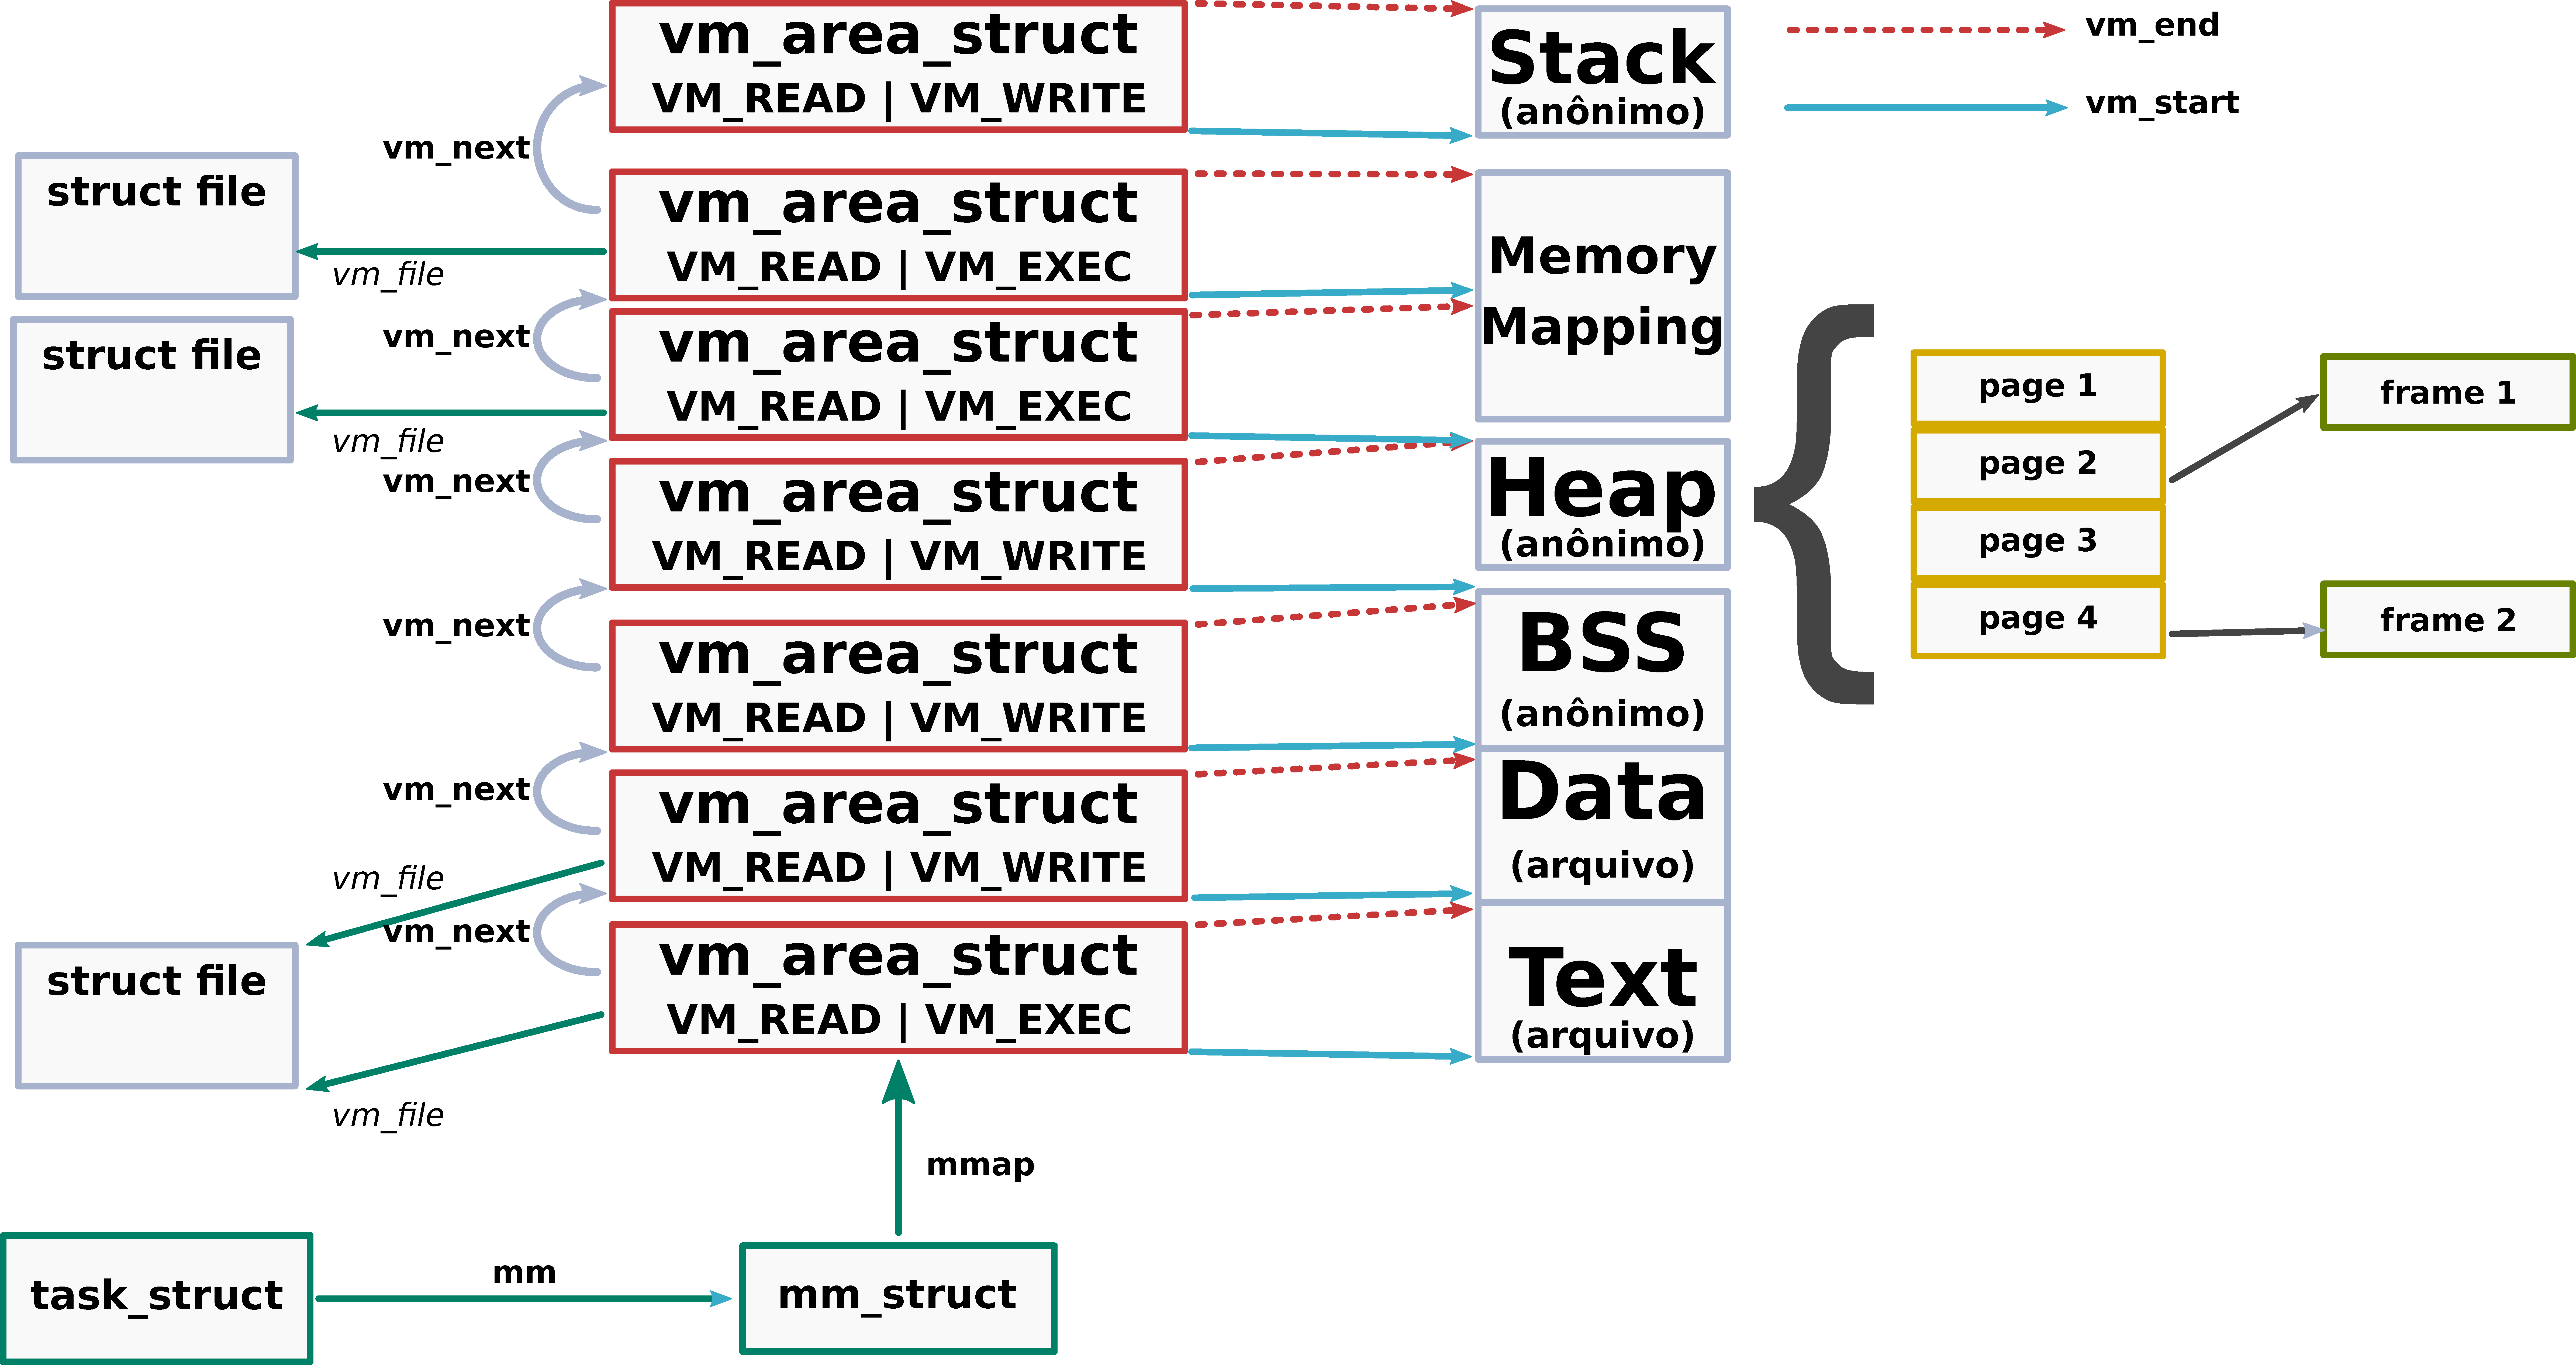
\includegraphics[width=\textwidth]{kernel_manages_memory}
  \caption{Visão interna do gerenciamento da memória, imagem baseada em \citep{kernel_manages_memory}}
  \label{fig:kernel_manages_memory}
\end{figure}

Para entender na prática como o Kernel gerencia a memória, vamos expandir os
conceitos da Figura X para a forma como eles são implementado no Linux. Veja a
Figura \ref{fig:kernel_manages_memory} ilustrando as estruturas de dados usadas
pelo Linux e as suas ligações. No Kernel a estrutura responsável por manter
todas as informações do processo (i.e.; PCB) chama-se \texttt{task\_struct},
essa tem um ponteiro para outra estrutura de dados chamada de
\texttt{mm\_struct}; por sua vez tal estrutura de dados mantém uma lista ligada
para estruturas do tipo \texttt{vm\_area\_struct} (ou \boldAndIndex{virtual memory
area - VMA}). A VMA em conjunto com a tabela de páginas orquestram o
gerenciamento do programa na memória.

Uma VMA consiste de um intervalo de endereços virtuais contíguos e sem
sobreposição com algumas \textit{flags} de controle de acesso associado a si. A
informação se a VMA é anonima ou não, vem do campo \texttt{vm\_file} (se esse
estiver vazio, então a área é anonima). Repare na figura que cada segmento
corresponde a uma VMA com exceção do segmento de mapeamento que pode ter mais.

Lembre-se que a VAS é dividia em páginas, por esse motivo o tamanho de uma VMA
deve ser um múltiplo de uma página. Toda vez que um acesso na memória é feito,
a tabela de páginas do processo é consultada e cada entrada dessa tabela é
descrita por uma série de metadados que descreve a região de memória. Cada
entrada recebe o nome de \boldAndIndex{entrada da tabela de páginas} (\textit{Page
Table Entry}) ou simplesmente PTE. A Figura \ref{fig:pte} ilustra como a
entrada é representada. Sem entrar em detalhes nos campos (a figura é
autoexplicativa), podemos concluir que uma página virtual é a unidade de
proteção da memória por que todos os bytes dela compartilham os bits User/Root
e Leitura/Escrita.

\begin{figure}[!h]
  \centering
  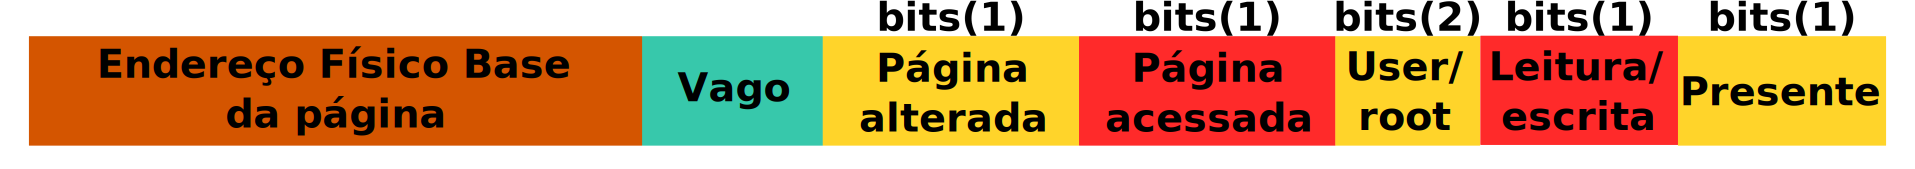
\includegraphics[width=\textwidth]{pte}
  \caption{Entrada da tabela de páginas}
  \label{fig:pte}
\end{figure}

Por fim para exemplificar como esses mecanismos estão relacionados, veja a
Figura \ref{fig:malloc_linux}. Nesse exemplo, temos um programa com algumas
paginas já mapeada para uma memória física. A aplicação decide alocar mais
memória por meio da função \texttt{malloc()}, por sua vez, uma chamada para
\texttt{brk()} é feita e o kernel atualiza o VMA do \textit{heap} com o tamanho
solicitado e retorna o ponteiro. Na prática, nenhum endereço físico foi alocado
e enquanto o programa não acessar a região alocada nenhum frame é criado. Na
primeira tentativa de acesso ocorre uma falha de página e a função
\texttt{do\_page\_fault()} é chamada. Se o processo atender as permissões
indicadas na PTE, então o kernel aloca e associa o frame a página.

\begin{figure}[!h]
  \centering
  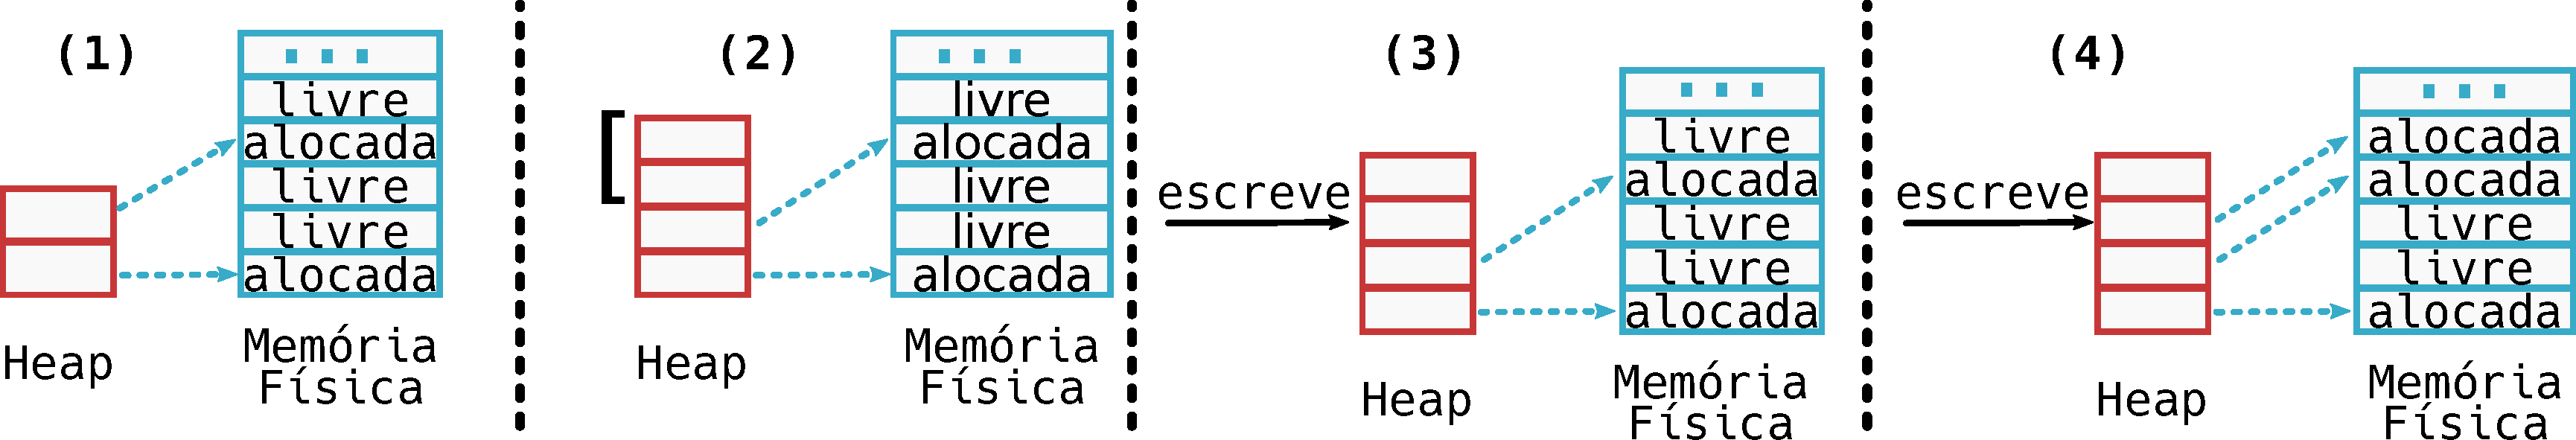
\includegraphics[width=.70\textwidth]{malloc}
  \caption{Alocação de memória com \texttt{malloc()}, imagem baseada em \citep{anatomy_program_mem}}
  \label{fig:malloc_linux}
\end{figure}

\section{Aspectos gerais relativos a abstração de processos}

\subsection{Chamadas de Sistema}
% TODO: Fazer a distinção entre user space e kernel space
% TODO: Falar do SYSCALL e VMSYSCALL - Atualizar o Dune

\cite{silberschatz} apresenta diversas perspectivas sobre os SOs, dentre elas
destaca-se a ideia de que um SO fornece serviços para tornar as tarefas de
programação mais simples para os desenvolvedores. Partindo de tal concepção
podemos notar os seguintes serviços: controle sobre a execução de um programa,
operações de I/O, manipulação de sistemas de arquivos, comunicação, detecção de
erros, alocação de recursos, dentre outros. Dado a vasta quantidade de serviços
oferecidos, deve-se ter a seguinte pergunta em mente: qual mecanismo utilizado
pelo SO para dar acesso para todos os serviços? A resposta é simples: chamadas
de sistema (também conhecidas por \emph{system call} ou \emph{syscall}).

De forma geral, podemos dizer que uma chamada de sistema consiste em uma API de
baixo nível que permite que uma aplicação executando no espaço de usuário
(\emph{user space}) faça uma requisição de baixo nível para o SO. Por sua vez,
esse pedido é rigorosamente validada pelo SO que pode permitir executar a
operação até o fim, retornando o que a aplicação solicitou; ou pode negar caso
encontre uma inconsistência. Na prática, esse tipo de operação consiste em uma
simples chamada de função que é tratada pelo SO. Normalmente cada
\emph{syscall} tem um número associado a si, com isso o SO consulta uma tabela
que identifica a função que deve ser chamada. Além disso, passar parâmetros
para esse tipo de função pode depender da arquitetura e de outros detalhes.
Para tentar esconder toda a complexidade por trás desse tipo de operação,
muitas vezes são escritas bibliotecas que encapsulam esse tipo de chamada. O
exemplo mais emblemático é a \emph{libc} que oculta vários detalhes de baixo
nível como a leitura e escrita de um arquivo.

Para ilustrar como esse conceito funciona na prática, veja a Figura
\ref{fig:userspace_kernelspace} mostrando um simples programa que pede o seu
PID para o SO (exemplo baseado em \cite{syscallex}). O programa executando está
na memória e esse tem o seu \emph{Address Space} devidamente inicializado; ao
invocar a função \texttt{getpid()}, o seu fluxo de execução é levado para a
\emph{libc}. Por sua vez a \emph{libc} faz algumas operações, tal qual alocar
espaço na memória para fazer cache do PID. Quando a \emph{libc} estiver pronta
ela finalmente faz a chamada para o sistema. Note que nessa etapa ocorre uma
mudança de um modo de execução menos privilégiado (\emph{ring 3}) para um modo
privilégiado (\emph{ring 0}). Nesse momento o SO tem total controle sobre o
pedido feito e faz a verificação dos parâmetros e permissões. Se tudo ocorrer
bem, o SO se encarrega de copiar a informação pós-processada do \emph{Kernel
space} para o \emph{user space}. Por fim, a \emph{libc} salva o valor do seu
cache evitando a necessidade do SO intervir no futuro e a aplicação finalmente
recebe o seu PID.

\begin{figure}[!h]
  \centering
  \includegraphics[width=0.8\textwidth]{userspace_to_kernel} 
  \caption{Execução do user space até o kernel space}
  \label{fig:userspace_kernelspace}
\end{figure}

\subsection{Troca de Contexto}

Em um SO de proposito geral é comum que tenhamos múltiplos processos executando
por um intervalo de tempo e após tal intervalo os processos são trocados. A
troca tem início quando uma interrupção ocorrer, seja ela porque o tempo de CPU
do processo terminou ou por qualquer outro motivo. O primeiro passo necessário
consiste em salvar todos o estado do processo em execução e em seguida carregar
o estado do novo processo na CPU. Repare que o tempo gasto na troca de processo
não produz nenhum trabalho útil sendo um mecanismo de
\textit{overhead}~\citep{silberschatz}.

Na prática a troca de contexto é bem mais complexa, por exemplo, vamos olhar de
perto e de forma breve a troca de contexto no GNU/Linux em uma arquitetura x86.
Primeiramente, todos os processos precisam compartilhar os registradores da
CPU, por esse motivo o kernel deve assegurar que todos os registradores sejam
carregados com os valores de quando o processo foi suspenso. O conjunto de
todos os dados dos registradores que devem ser carregado recebem o nome de
\boldAndIndex{contexto de hardware}~\citep{entendendo_kernel}, esse pode ser
visto como subconjunto do contexto do processo. No Linux o contexto do hardware
é armazenado na própria estrutura do processo e as demais partes são salvas na
stack do kernel mode. Toda troca de processo precisa armazenar o contexto de
hardware, por isso a \texttt{task\_struct} incluí um campo chamado de
\texttt{thread\_struct} que armazena o contexto do hardware (note que essa é
dependente da arquitetura de hardware).

Para realizar a troca de processos, o Kernel Linux realiza duas
operações~\citep{entendendo_kernel}:

\begin{enumerate}
  \item Instalar o novo espaço de endereço;
  \item Mudar o stack do Kernel mode e o contexto de hardware
\end{enumerate}

A operação de troca é extremamente dependente da arquitetura de hardware, pois
precisa ser executada de forma rápida e por isso o Linux tenta tirar proveito
de todo recurso disponibilizado pela CPU. Note que é preciso levar em
consideração os registradores que lidam com pontos flutuantes o que faz a troca
de contexto ainda mais complexa.

% Falar de PCID?
\subsection{Descritores de Arquivo}

Quando falamos de abstrações de processos é preciso levar em consideração
diversos aspectos interligado a eles, dentre eles as interações de escrita e
leitura de aquivos. Normalmente, quando um processo deseja ler ou escrever um
dado em um arquivo esse precisa passar por algumas camadas. De forma geral o
processo interage com o \boldAndIndex{sistema de arquivos} que é responsável
por fornecer um mecanismo simplificado para o processo localizar, escrever e
recuperar dados. Por sua vez, os sistemas de arquivos atuam com outras camadas
responsáveis por manter a organização e meta-dados sobre dos aquivos. Por fim,
as operações de alto nível são convertidas para instruções de baixo nível
passadas para os discos que de fato realizam as operações solicitadas.

Existe uma estrutura de dados utilizada para controlar o bloco de dados e que é
usada para leitura ou escrita, essa estrutura recebe o nome de
\boldAndIndex{inode}. Um inode contém diversas informações, dentre elas:
permissão, datas, dono do arquivo, tamanho, dentre outros. Quando um arquivo é
criado, uma estrutura de dados como o inode é criada e então o arquivo é salvo.

Quando um processo abre um arquivo, ele faz uma chamada para \texttt{open()}, em
seguida, o sistema de arquivos é acionado para encontrar o arquivo solicitado.
Para isso o \texttt{open()} primeiro procura em uma \boldAndIndex{tabela global
de arquivos} para verificar se o arquivo solicitado já está aberto. Se o
arquivo estiver presente na tabela global, então uma nova entrada em uma
\boldAndIndex{tabela local de arquivos dos processos} é feita e nela é
armazenada uma nova entrada com a posição referente ao arquivo na tabela
global. A tabela global é atualizada com a informação de que um novo processo
abriu o arquivo, basicamente um contador é incrementado para representar tal
informação . Por outro lado, se não existe uma entrada para o arquivo
solicitado na tabela global, então o mesmo é carregado e a tabela global
atualizada. A Figura \ref{fig:descritores} ilustra a operação descrita.
 
\begin{figure}[!h]
  \centering
  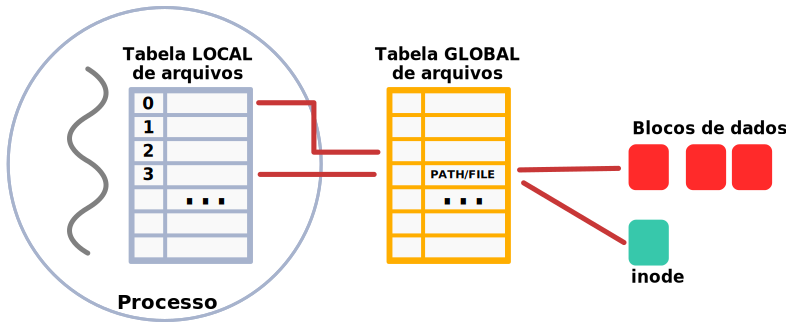
\includegraphics[width=.90\textwidth]{descritores} 
  \caption{Tabela local e global de arquivos}
  \label{fig:descritores} 
\end{figure}

Quando um arquivo é aberto por meio da função \texttt{open()}, esse retorna um
número chamado de \boldAndIndex{descritor de arquivo (file descriptor - fd)}
que nada mais é do que a posição da entrada na tabela local de processos.
Quando o processo fecha um arquivo, a entrada na tabela local é removida e o
contador de processos presente na tabela global é decrementado. Quando o
contador zera, o bloco é atualizado.

\subsection{Modelos de programação}

Além da manipulação de dispositivos de hardware, os SOs fornecem vários
recursos adicionais para o espaço de usuário, tal qual \emph{file locking} e
primitivas de segurança. Para fazer uso de tais recursos, a aplicação precisa
ser capaz de acessar as mesmas por meio de um modelo de programação coerente,
i.e., um conjunto bem estabelecido de abstrações interligadas. Um dado SO
implementa o seu modelo de programação dentro da sua própria API. Por exemplo,
tanto o GNU/Linux quanto Windows fornecem diferentes APIs de \emph{threading}
(\emph{pthread} e \emph{WindowsThreads}), mas ambos corresponde ao modelo de
programação de paralelismo.

Atualmente, a maioria dos SOs dão suporte para um grande número de modelos de
programação e suas respectivas APIs. Contudo, as aplicações mudam ao longo dos
anos e criam demandas para melhorias em áreas como camadas de segurança, opções
de otimizações e simplificação de código; esses aspectos são problemas reais.
Nesse sentido, propostas para expandir as abstrações de processos visando
introduzir novos modelos de programação são recorrentes e representam uma
interessante área para inovações.

%TODO: Mudar esse nome para algo melhor
\subsection{Aspectos de implementação}

As abstrações de processos são o ponto central no projeto de um SO moderno,
mapeando outras abstrações para ele; assim, outros serviços são suportados pelo
SO com a intenção de fornecer os mecanismos necessários para orquestrar todas
as operações dos processos (e.g., escalonador e gerenciamento de memória). Toda
estrutura necessária para gerir processos tem o lado negativo de utilizar CPU
(\emph{overhead}); para tentar mitigar essa situação, os SOs empregam um vasto
número de otimizações de hardware e software.

Mudanças em uma abstração de processos normalmente têm impactos no desempenho e
as consequências podem variar de acordo com a proposta de modificação. Por
exemplo, uma verificação adicional em uma camada pode elevar a sobrecarga no
sistema devido a uma nova característica implementada. Contudo, enquanto
extensões de processos podem degradar o desempenho, mas também podem trazer
benefícios de desempenho explorando alguma característica do hardware.

\subsection{Gerenciamento de Recursos}

Toda aplicação executando em um SO consome recursos do sistema. Frequentemente,
eles realizam boa parte do trabalho no espaço de usuário, o que requer pouca
intervenção do SO. Por exemplo, uma aplicação que faz cálculos complexos não
precisa de muito intervenção do SO. Contudo, existe uma grande quantidade de
software que demandam significante participação do SO para atingir os seus
objetivos, estendendo assim o seu consumo de recursos para o sistema. Por
exemplo, uma aplicação que utiliza recursos de rede tem várias partes das suas
atividades conduzidas pelo SO quando um pacote chega. Essa situação pode gerar
problemas devido ao controle indireto e descontrolado do uso de recursos por
atividades não confiáveis ao Kernel. Ataques do tipo \emph{Denial-of-service}
representam um exemplo da vida real que elevam o consumo do uso de recursos por
parte do SO.



\section{Device Drivers}
\label{sec:dd}

Um SO é repleto de elementos que buscam manipular e oculta a complexidade de
lidar com o hardware, portanto, tal software é consideravelmente grande e
complexo. Para tornar esse cenário ainda mais desafiador é preciso levar em
consideração que um SO deve fornecer suporte para uma infinidade de
dispositivos; a forma como os \emph{drivers} interagem com o Kernel deve ser
projetada com muito cuidado visando reduzir a complexidade e acoplamento.  O
design adotado na maioria dos SOs, é uma abordagem flexível na qual o código
para um dispositivo é mantido isolado em um \emph{driver}.

O isolamento fornecido por um \emph{device driver} é interessante, uma vez que
esse fornece um mecanismo e não uma política \citep{ddbook}. Entenda por
mecanismo como a capacidade que deve ser fornecido e por política como a forma
que a capacidade deve ser usada. Esse separação é interessante pois limita o
que um \emph{driver} deve fazer e por sua vez simplifica a implementação do
mesmo. Um exemplo disto é o \emph{Direct Rendering Managemente} do Kernel
Linux, esse fornece várias capacidades, dentre elas, a operação de trocar
\emph{framebuffers} primários com secundários; contudo é a aplicação que deve
controlar tal operação.

Por fim, é interessante ressaltar que alguns sistemas fornecem a ideia de
\boldAndIndex{Módulos carregáveis} (\textbf{loadable modules}) que significa que em
tempo de execução é possível carregar um novo \emph{device driver}. Esse tipo
de funcionalidade torna o SO mais leve e facilmente configurável. Por fim, os
módulos são extremamente flexíveis do ponto de vista da implementação uma vez
que são um código separado do núcleo do SO, respeitam a interface definida pelo
mesmo.

\section{Virtualização}
\label{sec:virtualizacao}

% TODO: Eu acho que faltou introduzir alguns dos termos básicos logo no início
% contar um pouco como funciona e acertar a fluídez do texto
% TODO: Falar brevemente do KVM - Atualizar o Dune

A ideia de oferecer a abstrações de máquinas virtuais dentro de uma mesma
máquina é um aspiração de longa data como o emblemático trabalho de Popek e
Goldberg demonstra~\citep{popek}. Este foi publicado em 1974 indicando os
requisitos necessários para a terceira geração processadores fornecessem
virtualização completa. Neste período se tinha noção de algumas das vantagens
que a virtualização por software e hardware poderia entregar. Dentre as
inúmeras vantagens da virtualização destacam-se a possibilidade de executar
aplicações legadas de um SO antigo, recursos que facilitam o processo de
desenvolvimento de software, serviços de nuvem, \emph{checkpoints}, migração de
processos, isolamento, dentre outras.

O elemento central da virtualização é o \emph{Virtual Machine Monitor (VMM)}
(também conhecido como \boldAndIndex{hypervisor}) que é responsável por criar a
ilusão de múltiplas máquinas em um mesmo hardware físico~\citep{tanenbaum}.
Essas máquinas virtuais rodando sobre o mesmo hardware tem a capacidade de
executar diferentes SOs. Complementarmente a estes conceitos, existe a ideia de
máquina convidada (\emph{guest}) e máquina hóspede (\emph{host}). O primeiro
refere-se ao SO que está executando sobre o VMM e o segundo refere-se a máquina
que está executando sobre o hardware com privilégios.

Um dos objetivos da virtualização consiste em permitir que um SO inicialize
como se estivesse inicializando em uma máquina real. Para que isso seja
possível é preciso emular o hardware de forma que o \emph{guest} não perceba
que está em um mecanismo simulado; ao mesmo tempo este processo deve ocorrer de
forma eficiente. Em 1974, \cite{popek} sugeriram alguns requisitos para que os
hardware modernos dessem suporte completo para virtualização, esses conceitos
são amplamente implementados nos processadores modernos. Basicamente os autores
destacam que três dimensões que devem ser consideradas para fornecer a
virtualização completa no nível dos processadores: segurança, fidelidade e
eficiência.

No que tange o assunto segurança, o VMM deve ter total controle sobre os
recursos virtualizados. Uma opção é utilizar um interpretador que intercepta
cada instrução e realiza exatamente o que a instrução precisa. Algumas
instruções podem ser executadas diretamente, mas outras não, por exemplo, não
deve ser possível para a máquina \emph{guest} desativar as interrupções de toda
a máquina \citep{tanenbaum}. Para contornar tal situação, o o SO \emph{guest}
deve ter a ilusão de que as interrupções estão desativadas.

Do ponto de vista da fidelidade, o comportamento do programa executando na
máquina virtual deve comportar-se de forma idêntica a se estivesse executando
diretamente no hardware. Na prática existem várias complicações associadas a
este requisito que levam a categorização das instruções utilizadas pela CPU em
três grupos de diferentes:

\begin{itemize}
  \item \boldAndIndex{Instruções sensíveis}: CPUs que fornecem \emph{user mode} e
        \emph{kernel mode} apresentam instruções comuns para ambos os modos de
        operação, mas que tem comportamentos diferentes dependendo de cada modo
        de operação no qual a instrução é executada;
  \item \boldAndIndex{Instruções privilégiadas}: São instruções que geram uma
        \emph{trap} quando executado no modo usuário, mas que não geram
        \emph{trap} em modo Kernel;
  \item \boldAndIndex{Instruções de controle de fluxo sensíveis}: São aquelas que
        tentam mudar a configuração de algum recurso do sistema.
\end{itemize}

Se você tentar fazer algo em modo usuário que você não deveria ser capaz de
fazer, o hardware deve capturar essa ação; em outras palavras, Popek e Goldberg
mostraram que uma máquina é virtualizavel se o conjunto de instruções sensíveis
é um subconjunto das instruções privilégiadas. Apesar de parecer um conceito
simples, levaram-se vários anos para que as CPUs incorporassem tais definições
e assim oferecessem um adequado suporte de hardware para a virtualização.

O suporte completo para a virtualização em hardware foi resolvido apenas em
2005 pela Intel \citep{uhlig} com uma tecnologia chamada \boldAndIndex{Virtualization
Technology (VT-x)}. A AMD tem uma solução parecida chamada \boldAndIndex{Secure
Virtual Machine (SVM)}. A ideia básica é criar um invólucro no qual a máquina
virtual pode executar um SO \emph{guest} iniciado dentro deste recipiente, o SO
contínua lá até que provoque uma \emph{trap} que faz com que o VMM tenha que
lidar com a situação. O conjunto de instruções que provocam uma \emph{trap} são
controlados por um conjunto de bits na qual o VMM tem acesso, essa extensão
torna possível a execução clássica de uma máquina virtual baseada em
"interrupção-e-emulação" \citep{tanenbaum}.

Do ponto de vista da eficiência, a virtualização deve fazer com que a maior
parte do código executado pelo SO \emph{guest} não sofra interferência do VMM.
Uma das abordagens utilizada antes de se ter o hardware de virtualização foi a
adoção de técnicas na qual o \textit{hypervisor} interceptava as instruções e
as reescrevia em tempo de execução com uma sequência de código considerada
segura.
Esse mecanismo permitia substituir instruções sensíveis, mas não privilégiadas;
tal técnica ficou conhecida como \boldAndIndex{tradução binária} e demostrou-se
extremamente eficiente devido ao seu sofisticado mecanismo de \emph{cache}.

% TODO: Falar dos tipos de hypervisor
%FIGURA X

\subsection{A tecnologia VT-x}
\label{sec:vtx}

Em 2005 Uhlig \citep{uhlig} apresentaram a tecnologia de virtualização adotada
pela Intel para fornecer a virtualização completa no nível do processador. Na
Figura \ref{fig:vt-x_flow} podemos notar os elementos presentes em tal
tecnologia e como eles interagem, dois novos modos de operações foram
introduzidos nas CPUs: \emph{VMX non-root} e \emph{VMX root}.

\begin{figure}[!h]
  \centering
  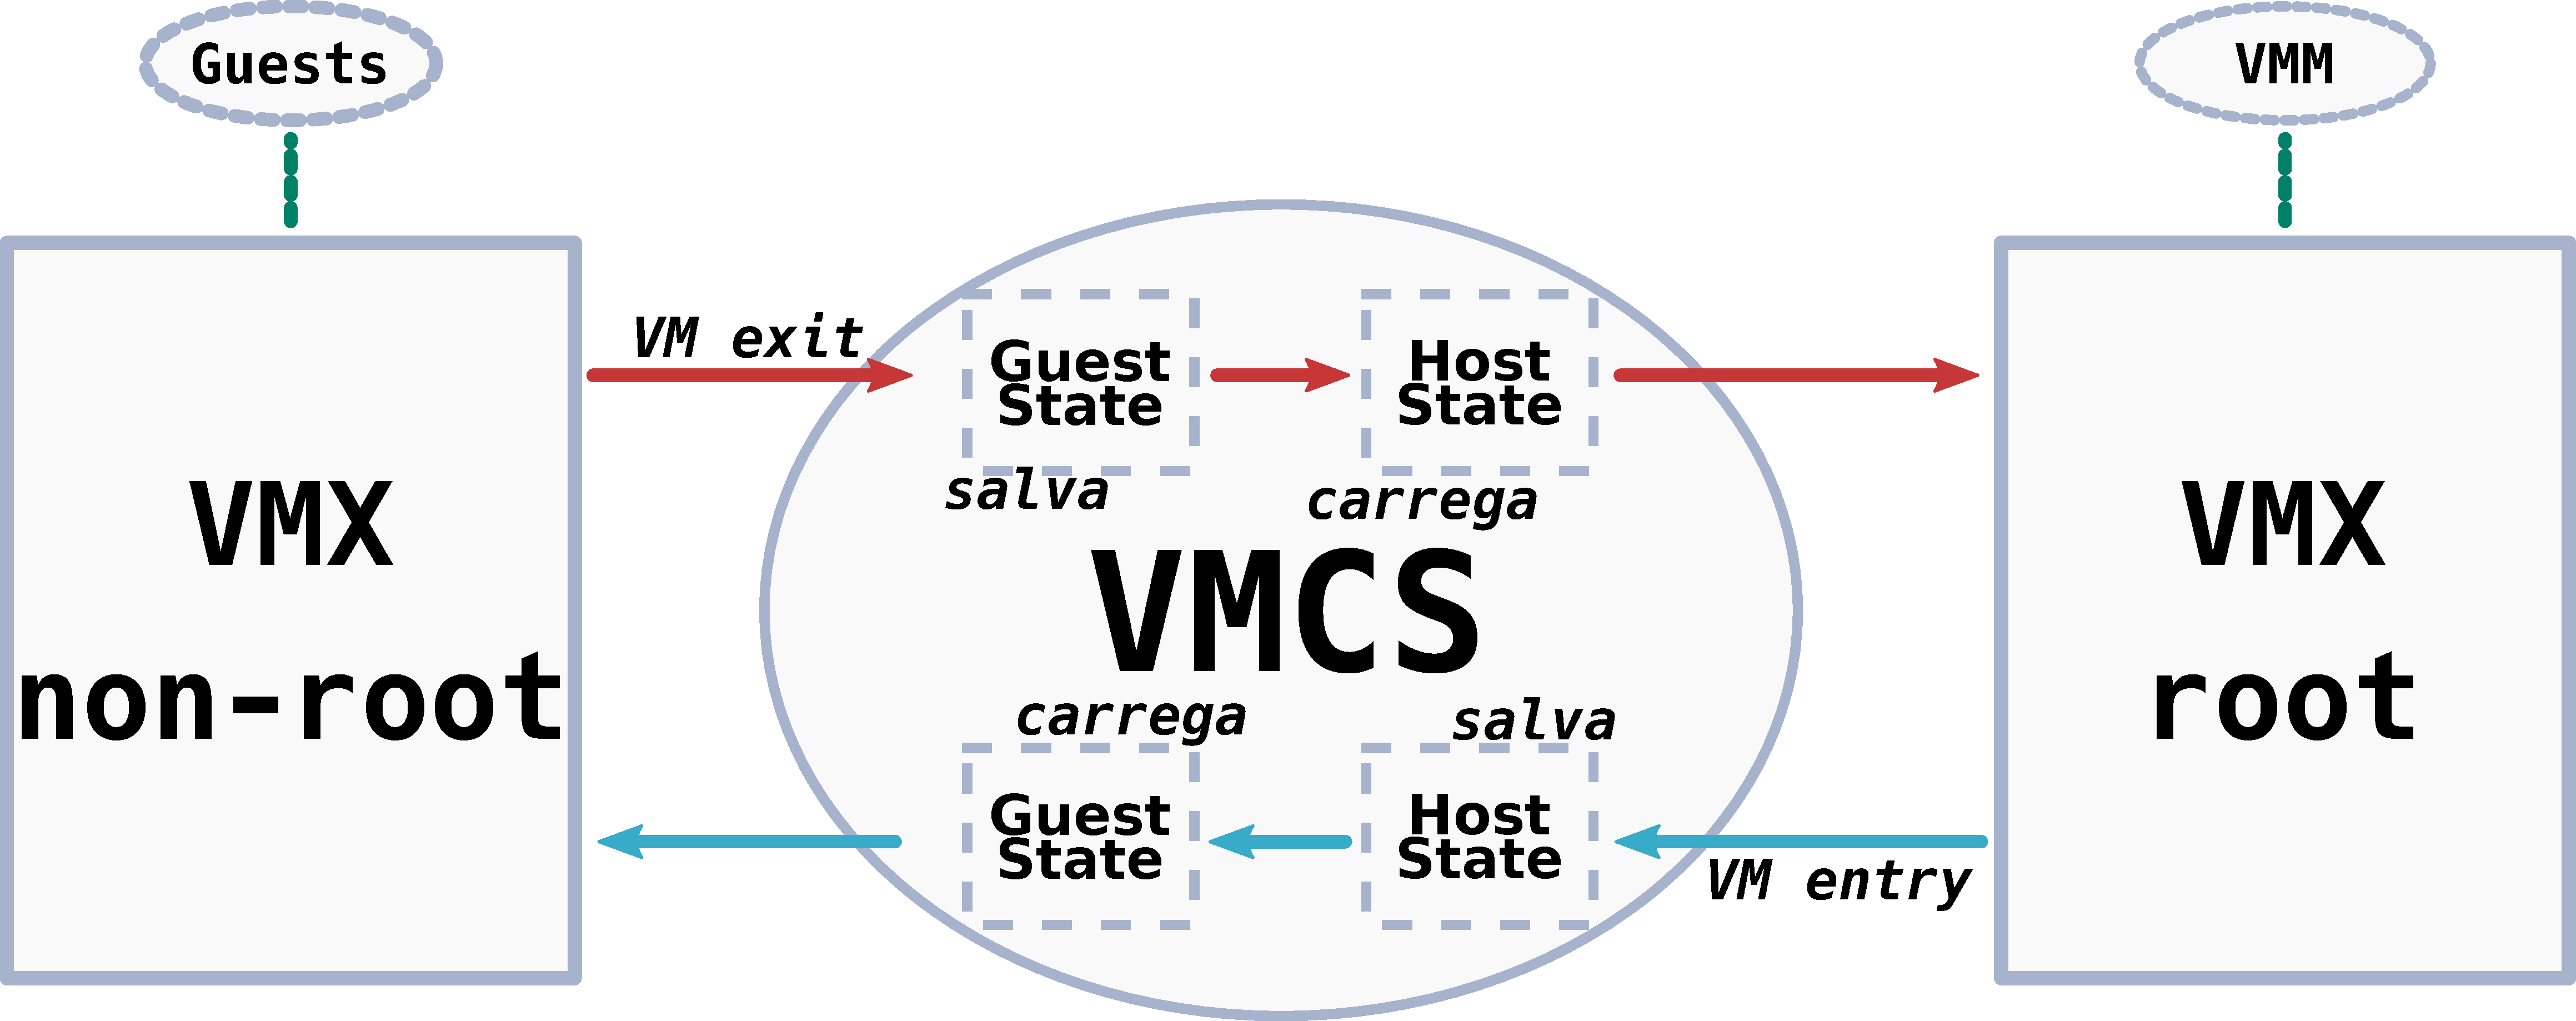
\includegraphics[width=0.6\textwidth]{vt-x_flow} 
  \caption{Fluxo do comportamento da tecnologia VT-x}
  \label{fig:vt-x_flow}
\end{figure}

O \emph{VMX non-root} é o modo de operação na qual a máquina \emph{guest}
executa, enquanto o \emph{VMX root} é o modo de operação utilizado pelo VMM. É
interessante observar que os dois modos tem suporte para os quatro níveis de
privilégios fornecidos pelos processadores Intel, isto permite que a máquina
\emph{guest} que tente executar uma instrução privilégiada em algum desses
nível forneçam tal informação para o VMM. Contudo, os software executando como
\emph{VMX non-root} são desprivilegiados de certa forma, a não pelo nível de
privilégios. Note da Figura \ref{fig:vt-x_flow} que existe uma transição chamada
\emph{VM exit} e \emph{VM entry}. A transição \emph{VM exit} ocorre quando o
controle é transferido do \emph{guest} para o VMM, isto faz com que o estado da
máquina \emph{guest} seja salvo e o estado do \emph{host} seja carregado para
que o VMM decida como tratar a interrupção. No sentido oposto, ocorre a
transição \emph{VM entry} na qual o VMM transfere o controle para a máquina
\emph{guest}, para isto ela salva o estado do \emph{host} e carrega o estado
anterior do \emph{guest}. Todas as informações referentes a virtualização são
mantidas em uma estrutura de dados chamadas de \emph{virtual-machine control
structure (VMCS)} que basicamente tem por função gerenciar as transições entre
a \emph{VM entry} e \emph{VM exit}.

